% Copyright (c) 2023 Ludovic Lars
% This work is licensed under the CC BY-NC-SA 4.0 International License

\chapter{Le consensus par le minage}
\label{ch:confirmation}
\label{enotezch:8}

\lettrine[]{B}itcoin est un modèle décentralisé de monnaie numérique issu de l'informatique distribuée, une discipline développée au moment de l'émergence d'Internet. Il se fonde plus précisément sur un réseau pair à pair d'ordinateurs, dans lequel les participants possèdent tous les mêmes responsabilités. En tant que tel, il constitue un \emph{système d'argent liquide électronique pair à pair}.

Tout l'enjeu de Bitcoin est ainsi de se mettre d'accord sur le contenu d'un registre déterminant qui possède quoi, c'est-à-dire d'arriver à un consensus sur la propriété des unités. En particulier, l'établissement d'un tel accord permet de résoudre le problème de la double dépense, qui se pose dans le monde numérique en raison de la facilité de reproduction des données.

Le consensus -- accord unanime au sein d'un groupe de personnes -- n'est pas une chose facile à atteindre entre les êtres humains. La conciliation sociale peut fonctionner concernant des règles générales, mais n'est pas adaptée quant aux détails particuliers. C'est pourquoi les organisations humaines sont bien souvent obligées de s'en remettre à une autorité centrale chargée de prendre les décisions.

Bitcoin a précisément pour contrainte d'éviter le recours à un tiers de confiance. Il utilise à cette fin un mécanisme de consensus distribué et ouvert, qui repose sur une activité appelée communément le minage, où la confirmation des transactions, c'est-à-dire leur inclusion dans le registre, est assurée par un procédé nommé la preuve de travail. Dans ce chapitre, nous détaillerons le fonctionnement de cet algorithme de consensus novateur.

% De ce fait, il repose sur un mécanisme de consensus distribué, que l'on appelle communément le minage, où la confirmation des transactions, c'est-à-dire leur inclusion dans le registre, est assurée par un procédé nommé la preuve de travail.

% Le minage, en plus d'être la manière dont sont distribués les nouvelles unités (d'où son nom), est le moyen par lequel le réseau arrive à un consensus.

\section*{Le problème des généraux byzantins} % Le consensus distribué
\addcontentsline{toc}{section}{Le problème des généraux byzantins}

% --- Métaphore des généraux byzantins ---

L'enjeu du consensus est illustré par le problème des généraux byzantins, qui est un problème d'informatique distribuée formalisé en 1982 par Leslie Lamport, Robert Shostak et Marshall Pease\sendnote{Leslie Lamport, Robert Shostak, Marshall Pease, «~\eng{The Byzantine Generals Problem}~», in \eng{ACM Trans. Program. Lang. Syst.}, vol.~4, no.~3, 1982, pp.~382–-401~: \url{https://lamport.azurewebsites.net/pubs/byz.pdf}.}. Ce problème traite de la remise en cause de la fiabilité des transmissions et de l'intégrité des participants dans les systèmes distribués, et il s'applique dans les cas où les composants d'un système informatique ont besoin d'être en accord.

Le problème est énoncé sous la forme d'une métaphore faisant intervenir des généraux de l'armée de l'Empire byzantin, l'Empire romain d'Orient qui a subsisté jusqu'en 1453 suite à la chute de la partie occidentale en 476\sendnote{Selon Leslie Lamport, l'appellation byzantine a été choisie pour ne pas offenser le sentiment patriotique du lecteur (l'armée dans la métaphore comporte des traîtres), car cette appellation a été faite \emph{a posteriori} par les historiens et les Byzantins eux-mêmes se considéraient comme romains. -- Voir Leslie Lamport, \eng{My Writings}~: \url{http://lamport.azurewebsites.net/pubs/pubs.html\#byz}.}. Ces généraux assiègent une ville ennemie avec leurs troupes dans le but de l'attaquer. Ils ne peuvent communiquer qu'à l'aide de messages relayés oralement et ils doivent trouver un moyen d'établir un plan de bataille commun par ce moyen. Par exemple, les généraux peuvent chercher à coordonner une attaque à l'aube, et partagent leurs intentions entre eux en envoyant le message «~attaque~» par le biais d'un message pour confirmer l'assaut, et «~retraite~» pour l'annuler. % Le nom de cet empire fait référence à Byzance, le nom antique de sa capitale Constantinople (aujourd'hui Istanbul).

% La situation est la suivante. Des généraux de l'armée byzantine campent autour d'une cité ennemie avec leurs troupes et souhaitent l'attaquer. Ils ne peuvent communiquer qu'à l'aide de messagers oraux et doivent établir un plan de bataille commun. Pour prendre un exemple simple, les généraux peuvent chercher à coordonner une attaque à l'aube, et partagent leurs intentions entre eux en envoyant le message «~attaque~» pour confirmer l'assaut, et «~retraite~» pour l'annuler.

Cependant, un petit nombre de ces généraux s'avèrent être des traîtres au service de l'ennemi qui essaient de semer la confusion au sein de l'armée. Ces traîtres envoient ainsi des messages contradictoires à leurs interlocuteurs, pour faire en sorte que certains généraux loyaux attaquent, et que d'autres battent en retraite au moment de l'assaut, causant par là une défaite certaine, comme illustré sur la figure~\ref{fig:byzantine-generals-attack}.

\begin{figure}[h]
  \centering
  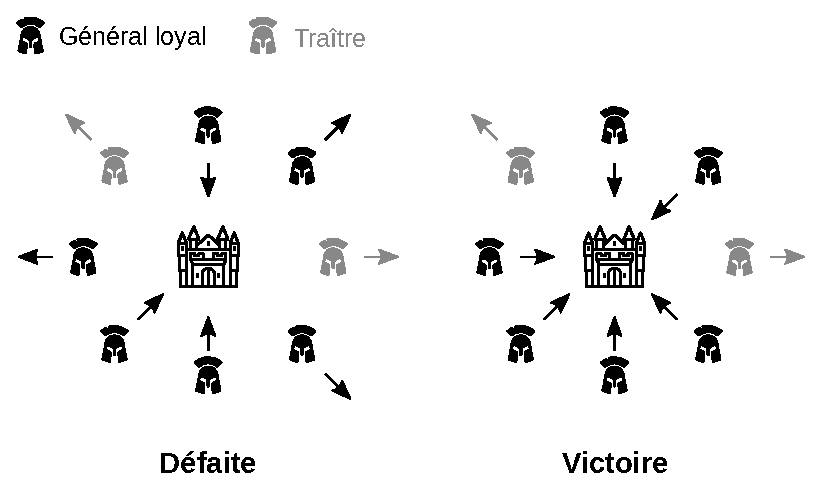
\includegraphics[scale=0.7]{img/byzantine-generals-attack.eps}
  \caption{Attaque des généraux byzantins contre la ville~: succès et échec.}
  \label{fig:byzantine-generals-attack}
\end{figure}

Le problème est de trouver une stratégie (c'est-à-dire un algorithme) permettant de s'assurer que tous les généraux loyaux se mettront d'accord sur le plan de bataille. Les traîtres battront alors en retraite, mais puisque leur nombre est supposément restreint, l'attaque sera quand même un succès.

La situation fait qu'il est difficile de parvenir à un consensus. On ne peut pas désigner un commandant auquel les généraux subordonnés obéiront, car le commandant peut être lui-même un traître. Lamport, Shostak et Pease ont montré que le problème peut être résolu de manière absolue si (et seulement si) les généraux loyaux représentent strictement plus des deux tiers de l'ensemble des généraux\sendnote{Cette propriété est démontrée dans l'article original de Lamport et al. La condition plus précise est $n \ge 3 m + 1$ où $n$ est le nombre total de généraux et $m$ le nombre de traîtres.}~; autrement dit, qu'il ne peut pas y avoir plus d'un tiers de traîtres au sein de l'armée.

% Abstract: "Reliable computer systems must handle malfunctioningcomponents that give conflicting information to different parts of the system. This situation can be expressed abstractly in terms of a group of generals of the Byzantine army camped with their troops around an enemy city. Communicating only by messenger, the generals must agree upon a common battle plan. However, one or more of them may be traitors who will try to confuse the others. The problem is to find an algorithm to ensure that the loyal generals will reach agreement. It is shown that, using only oral messages, this problem is solvable if and only if more than two-thirds of the generals are loyal; so a single traitor can confound two loyal generals. With unforgeable written messages, the problem is solvable for any number of generals and possible traitors. Applications of the solutions to reliable computer systems are then discussed."

% --- Application de la métaphore aux systèmes distribués ---

La métaphore des généraux byzantins s'applique directement aux systèmes distribués, c'est-à-dire aux systèmes dont les composants sont séparés et doivent communiquer les uns avec les autres pour se synchroniser. Les généraux représentent les composants du système, les traîtres les composants défaillants, et les messages les données transmises entre les composants. Le but est d'obtenir un algorithme permettant de détecter les défaillances, appelées pannes byzantines, et de permettre aux autres composants de les écarter. La résilience obtenue est appelée la tolérance aux pannes byzantines~; le système est dit BFT, pour \eng{Byzantine Fault Tolerant}.

Le problème a été initialement décrit pour les systèmes informatiques reposant sur des composants présents à différents endroits et dans lesquels la bonne transmission des données est critique, comme les systèmes aéronautiques et spatiaux\sendnote{L'infrastructure du Boeing 777 repose notamment sur le bus informatique ARINC 629 qui réplique en quadruple les messages envoyés afin de garantir un résultat avec une latence très faible. -- Elaine Ou, \eng{Byzantine Fault Tolerant Airplanes}, 12 février 2017~: \url{https://elaineou.com/2017/02/12/byzantine-fault-tolerant-airplanes/}.}. Mais il concerne aussi (ce qui nous intéresse ici) les systèmes pair à pair reposant sur un réseau horizontal de participants, et en particulier les systèmes cryptoéconomiques comme Bitcoin, dans lesquels les nœuds du réseau ont besoin de se mettre d'accord sur le contenu d'un registre. L'objectif est alors de trouver un algorithme permettant à tous les nœuds honnêtes de parvenir à un consensus en présence de nœuds traîtres (dits «~byzantins~»).

% replicated state machine
% réplication de machine à état (state machine replication) 

% --- Algorithmes de consensus classiques ---

Avant Bitcoin, le problème était résolu par des algorithmes dits «~classiques~» basés sur les idées de Lamport, Shostak et Pease. Le plus connu est probablement l'algorithme de consensus PBFT (pour \eng{Practical Byzantine Fault Tolerance}), mis au point par Miguel Castro et Barbara Liskov en 1999\pagenote{«~l'algorithme de consensus PBFT [...] mis au point par Miguel Castro et Barbara Liskov en 1999~»~: Miguel Castro, Barbara Liskov, \eng{Practical Byzantine Fault Tolerance}, février 1999.}, qui permettait à un nombre donné de participants de se mettre d'accord en gérant des milliers de requêtes par seconde avec une latence de moins d'une milliseconde.

Bien avant Bitcoin, Wei Dai et Nick Szabo envisageaient d'utiliser ce type d'algorithme pour leurs systèmes de monnaie électronique, b-money et bit gold. De même, de nombreux systèmes cryptoéconomiques en font encore aujourd'hui usage pour des raisons de performance, à l'instar d'Ethereum dont le consensus est basé sur l'algorithme Casper FFG. % comme nous l'avons vu dans le chapitre~\ref{ch:cybermonnaie}

Cependant, ces algorithmes impliquent des contraintes fortes~: les nœuds doivent connaître l'ensemble des autres nœuds et ils doivent communiquer avec tous les autres. De ce fait, il faut sélectionner les nœuds ayant le droit de participer au consensus avant de lancer l'algorithme, ce qui se fait généralement par preuve d'autorité (\eng{proof of authority}), via une liste blanche de nœuds, ou par preuve d'enjeu (\eng{proof of stake}), via un montant d'unités possédées ou déléguées. Cela implique une moins bonne robustesse du système, car les validateurs sont alors connus de tous et donc davantage exposés aux attaques.

% La communication entre les nœuds du réseau doit être quadratique (chaque nœud doit communiquer avec tous les autres), ce qui fait qu'il est difficile de dépasser les 10 000 nœuds.

% --- Algorithmes de consensus de Bitcoin ---

Bitcoin résout ce problème d'une manière différente, grâce à un nouveau type d'algorithme~: l'algorithme de consensus de Nakamoto par preuve de travail. Celui-ci est plus robuste dans le sens où les nœuds du réseau n'ont pas besoin de connaître l'ensemble des autres nœuds et où aucune identification n'est requise.

Puisque le rôle principal de Bitcoin est le transfert de valeur, l'objectif est de se mettre d'accord sur qui possède quoi, c'est-à-dire sur l'\emph{état} du système. La solution proposée par Satoshi Nakamoto consiste à employer un registre recensant l'intégralité des transactions réalisées depuis le lancement du système, «~la seule façon de confirmer l'absence d'une transaction [étant] d'être au courant de toutes les transactions\sendnote{Satoshi Nakamoto, \eng{Bitcoin: A Peer-to-Peer Electronic Cash System}, 31 octobre 2008.}~». Ce registre formant l'\emph{historique} du système est organisé comme une succession de blocs de transactions, de sorte qu'il est communément appelé la \emph{chaîne de blocs}. Les nœuds du réseau entretiennent chacun une copie complète de la chaîne dont ils transmettent des éléments sur demande.

Les nouveaux blocs sont ajoutés à la chaîne de manière régulière grâce à la production d'une preuve de travail. Les acteurs réalisant cette opération sont appelés des mineurs. Les nœuds du réseau arrivent à un consensus en considérant que la chaîne la plus longue est la chaîne correcte. Ainsi, comme l'a écrit Satoshi Nakamoto~:

\vspace{-1em}
\begin{quote}
«~La chaîne de preuves de travail est une solution au problème des généraux byzantins\sendnote{Satoshi Nakamoto, \eng{Re: Bitcoin P2P e-cash paper}, \wtime{13/11/2008, 22:56:55 UTC}~: \url{https://www.metzdowd.com/pipermail/cryptography/2008-November/014849.html}.}.~»
\end{quote}

La spécificité novatrice de cet algorithme est qu'il résout le problème de manière probabiliste plutôt que de manière absolue\sendnote{Plus précisément, il s'agit de sacrifier un peu de la propriété de sécurité au sens de Lamport pour améliorer la tolérance aux pannes byzantines.}. Par conséquent, les transactions incluses dans le registre ne sont jamais strictement finales, mais sont (probabilistiquement parlant) considérées comme telles au bout d'un temps. Ce fonctionnement permet de n'avoir besoin que de 51~\% de validateurs honnêtes, au lieu des 67~\% requis par les algorithmes classiques.

% Il s'agit d'un système de comptabilité à triple entrée\sendnote{Ian Grigg, \eng{Triple Entry Accounting}, 25 décembre 2015~: \url{https://iang.org/papers/triple_entry.html}~; Ian Grigg, \eng{Is BitCoin a triple entry system?} 13 juin 2011~: \url{http://financialcryptography.com/mt/archives/001325.html}.}, où le mécanisme de consensus joue le rôle de la tierce partie chargée d'assurer les transactions réalisées entre deux utilisateurs.

% La solution est moins efficace mais plus robuste. 

\section*{La preuve de travail}
\addcontentsline{toc}{section}{La preuve de travail}

% --- Description et historique du procédé ---

La preuve de travail, de l'anglais \eng{proof of work}, est un procédé permettant à un appareil informatique de démontrer de manière objective et quantifiable qu'il a dépensé de l'énergie. Ce moyen est utilisé pour sélectionner les ordinateurs dans le cadre de l'accès à un service ou à un privilège.

La preuve de travail est un mécanisme de résistance aux attaques Sybil, qui rend difficile la multiplication des identités à l'excès par un acteur qui chercherait à prendre le contrôle du réseau. Une attaque Sybil\pagenote{«~attaque Sybil~»~: Voir John R. Douceur, «~\eng{The Sybil Attack}~», in \eng{Peer-to-Peer Systems}, 2002, pp. 251--260. La pratique a été décrite en 1993 par le cypherpunk L. Detweiler sous le nom de \eng{pseudospoofing}~: \url{https://cypherpunks.venona.com/date/1993/10/msg00760.html}.} est une attaque intervenant au sein d'un réseau ouvert basé sur un système de réputation qui consiste à dupliquer les profils à moindre coût pour en altérer le fonctionnement. C'est par exemple un problème particulièrement présent sur les médias sociaux, où les comptes de robots sont utilisés en masse pour augmenter la visibilité d'un contenu donné. % prendre le contrôle du réseau : ici la confirmation des transactions

Le concept de preuve de travail a été décrit pour la première fois par Cynthia Dwork et Moni Naor en 1992, dans un article visant à présenter une méthode permettant de combattre le courrier indésirable (\eng{spam}) dans les boîtes de réception\sendnote{Cynthia Dwork, Moni Naor, \eng{Pricing via Processing or Combatting Junk Mail}, 1992.}. Le terme «~\eng{proof of work}~» est quant à lui apparu en 1999 sous la plume de Markus Jakobsson et Ari Juels\sendnote{Markus Jakobsson, Ari Juels, \eng{Proofs of Work and Bread Pudding Protocols (Extended Abstract)}, 1999.}.

L'idée de Dwork et Naor a été implémentée par le cypherpunk britannique Adam Back en 1997 au moyen de Hashcash, un algorithme produisant de manière simple des preuves de travail avec une fonction de hachage, qui devait principalement servir pour le courrier électronique\sendnote{Adam Back, \eng{[ANNOUNCE] hash cash postage implementation}, \wtime{28/03/1997 16:52:26 UTC}~: \url{https://cypherpunks.venona.com/date/1997/03/msg00774.html}~; Adam Back, \eng{Hashcash -- A Denial of Service Counter-Measure}, 1\ier{} août 2002~: \url{http://www.hashcash.org/hashcash.pdf}.}. Cette implémentation a été reprise dans le système de preuves de travail réutilisables (RPOW) de Hal Finney mis en application en 2004. % Il s'agit également de l'algorithme utilisé dans le minage de Bitcoin.

% --- Description de Hashcash ---

L'algorithme de preuve de travail de Hashcash consiste à trouver une collision partielle de la fonction de hachage considérée, c'est-à-dire à obtenir deux messages ayant une empreinte commençant par les mêmes bits de données. À partir de la version 1.0 sortie en 2002, il s'agit plus précisément de découvrir une collision partielle pour l'empreinte zéro, à savoir trouver un antécédent dont l'empreinte commence par un nombre de zéros binaires déterminés. Puisque la fonction de hachage est à sens unique (résistance à la préimage), une telle obtention ne peut être réalisée qu'en testant une à une les différentes possibilités, ce qui demande de l'énergie. L'antécédent obtenu est appelé une preuve de travail.

La preuve de travail est réalisée par le calcul successif d'empreintes d'une chaîne de caractères, composée d'une information de base, et d'un nombre qu'on fait varier, appelé le compteur ou le nonce. L'information de base comporte généralement des indications sur le contexte dans lequel la preuve de travail a été produite (identifiant, date, heure, protocole,~etc.) pour démontrer que cette preuve de travail n'a pas déjà été utilisée.

Prenons un exemple pour illustrer le propos. D'abord, on choisit une information de base propre au contexte~: pour produire une preuve de travail liée à cet ouvrage et à sa date d'écriture, on peut opter pour l'information de base \longstring{20231031181000:BitcoinElegance:}. Puis on détermine le degré de la preuve de travail, c'est-à-dire le nombre de zéros binaires par lequel doit commencer l'empreinte, ici 16. On procède ensuite à la recherche du résultat voulu en incrémentant le nonce~: à chaque itération, on le met bout à bout avec l'information de base et on vérifie si l'empreinte de l'ensemble est satisfaisante. Le travail s'arrête enfin lorsque l'empreinte commence avec un nombre suffisant de zéros~: ici 95~690 tentatives. Notre preuve de travail est donc~:

\begin{Verbatim}[fontsize=\footnotesize]
20231031181000:BitcoinElegance:95690
\end{Verbatim}

Et l'empreinte correspondante, commençant par 4 zéros hexadécimaux (soit 16 zéros binaires), est~:

\begin{Verbatim}[fontsize=\footnotesize]
0000387b99b1412e3cb6e49548cc0d11bdc797138e1a0f5ff095279a710b895a
\end{Verbatim}

Les étapes de cette procédure sont décrites dans le tableau~\ref{table:hashcash-hashes}.

\begin{table}[h]
  \begin{tabular}{| c | c |}
    \hline \footnotesize \textbf{Nonce} & \footnotesize \textbf{Empreinte (SHA-256)} \\
    \hline \footnotesize 0 & \scriptsize \longstring{933c448c18e334c1cc5191f035d8581af611417578392b2d695d521c29b396d5} \\
    \hline \footnotesize 1 & \scriptsize \longstring{50530c98d1b171826b3d26fa5442e4ce7aa1f8a1277b71bc74d3adc1cd88b9ae} \\
    \hline \footnotesize 2 & \scriptsize \longstring{fa27ed560df22d676d69966c9a981c5adfc395b4e7f78ca54d2593a98fd2ea38} \\
    \hline \footnotesize 3 & \scriptsize \longstring{011692df53a84ecdddcd154de4f329e7311090580adb189e8360ea1729d75c99} \\
    \hline
    \hline \footnotesize 95~690 & \scriptsize \longstring{0000387b99b1412e3cb6e49548cc0d11bdc797138e1a0f5ff095279a710b895a} \\
    \hline
  \end{tabular}
  \caption{Recherche de la preuve de travail à partir de l'information de base \texttt{20231031181000:BitcoinElegance:}.}
  \label{table:hashcash-hashes}
\end{table}

% elegance.py
% Target                                0000ffff00000000000000000000000000000000000000000000000000000000
% 20231031181000:BitcoinElegance:0      933c448c18e334c1cc5191f035d8581af611417578392b2d695d521c29b396d5
% 20231031181000:BitcoinElegance:1      50530c98d1b171826b3d26fa5442e4ce7aa1f8a1277b71bc74d3adc1cd88b9ae
% 20231031181000:BitcoinElegance:2      fa27ed560df22d676d69966c9a981c5adfc395b4e7f78ca54d2593a98fd2ea38
% 20231031181000:BitcoinElegance:3      011692df53a84ecdddcd154de4f329e7311090580adb189e8360ea1729d75c99
% 20231031181000:BitcoinElegance:4      1d9142dc4c94efc7c8b061237f3f415782c019e102bf3771bc2b8aa1c69eafa9
% 20231031181000:BitcoinElegance:95690  0000387b99b1412e3cb6e49548cc0d11bdc797138e1a0f5ff095279a710b895a

Statistiquement, ce type de recherche implique d'essayer 65~536 possibilités ($2^{16}$) pour tomber sur une solution. En moyenne, la production d'une telle preuve de travail démontre donc qu'un effort approchant a été effectué. De plus, il existe une asymétrie entre la production et la vérification, cette dernière ne nécessitant qu'une seule application de la fonction de hachage et étant par conséquent peu coûteuse.

Le coût de production moyen confère une certaine rareté aux preuves de travail~: plus leur degré est élevé, plus elles sont difficiles à produire. D'où le fait qu'on puisse les utiliser en tant que marques de qualité pour le courrier électronique comme dans Hashcash, ou bien en tant que pièces monétaires de base comme dans bit gold et RPOW.

% --- Hashcash et Bitcoin ---

Le minage de Bitcoin intègre le procédé de preuve de travail de Hashcash sous la forme d'une variante~: l'objectif est de trouver une empreinte inférieure à une valeur cible précise, et non pas une empreinte commençant par un nombre de zéros déterminés. Ce procédé est appliqué entre les blocs de transactions, de sorte que ces blocs, ou plutôt leurs entêtes comme nous l'expliquerons plus bas, constituent eux-mêmes les preuves de travail.

Dans Bitcoin, le rôle de la preuve de travail est double~: exiger un coût pour la fabrication des nouveaux bitcoins et faire en sorte que le réseau puisse arriver à un consensus. D'une part, elle a pour but d'imposer la cherté de l'unité de compte. Cela rappelle les modèles qui ont précédé Bitcoin, et c'est pourquoi Hal Finney a été jusqu'à qualifier les bitcoins de «~jetons de preuve de travail\sendnote{Hal Finney, \eng{Bitcoin v0.1 released}, \wtime{24/01/2009 16:48:03 UTC}~: \url{https://www.metzdowd.com/pipermail/cryptography/2009-January/015036.html}.}~» (\eng{POW tokens}) en 2009. Toutefois, les bitcoins ne sont pas exactement des preuves de travail dans le sens où la difficulté de production est variable, évoluant selon la puissance de calcul totale déployée sur le réseau. Ainsi, mis à part dans le cas limite de la difficulté minimale du système, le but est de s'assurer que la production des unités demande de l'énergie, pas d'exiger un coût en travail fixe. D'autre part, la preuve de travail a pour objectif de garantir le consensus sur le réseau, en faisant en sorte que les nœuds honnêtes se mettent d'accord sur qui possède quoi. Elle limite l'accès à la production des blocs~: la sélection du validateur (mineur) se fait selon le montant d'énergie dépensé. La preuve de travail joue ici son rôle de défense contre les attaques Sybil en empêchant les attaquants de mettre en place un grand nombre de nœuds pour contrôler le système\sendnote{«~Si la majorité était basée sur le principe de vote par adresse IP (une adresse IP, une voix), elle pourrait être détournée par toute personne capable de s'octroyer de nombreuses adresses IP. La preuve de travail est essentiellement basée sur la puissance de calcul~: un processeur, une voix.~» -- Satoshi Nakamoto, \eng{Bitcoin: A Peer-to-Peer Electronic Cash System}, 31 octobre 2008.}.

Ce fonctionnement fait que la chaîne de blocs forme une chaîne de preuves de travail, qui récapitule l'ensemble du travail effectué depuis le début. De ce fait, la chaîne constitue un historique linéaire difficilement malléable comme nous le verrons.

\section*{La chaîne de blocs}
\addcontentsline{toc}{section}{La chaîne de blocs}

La chaîne de blocs, ou \eng{blockchain} en anglais, est la structure de données regroupant l'ensemble des transactions réalisées depuis le lancement du système. Cette structure est une suite de blocs de transactions, liés les uns aux autres par un procédé appelé l'horodatage.

% --- Horodatage ---

L'horodatage est une technique permettant d'associer une date et une heure à une information, qui a été décrite en 1991 par Stuart Haber et Scott Stornetta dans le cas particulier de l'horodatage de documents\pagenote{«~décrite en 1991 par Stuart Haber et Scott Stornetta dans le cas particulier de l'horodatage de documents~»~: Stuart Haber, Wakefield Scott Stornetta, «~\eng{How to time-stamp a digital document}~», \eng{Journal of Cryptology}, 1991~: \url{http://www.staroceans.org/e-book/Haber_Stornetta.pdf}.}. Le principe est simple~: il consiste à hacher une information (ou un document) et de partager l'empreinte obtenue pour prouver que l'information (ou le document) existait à la date de partage. Cette méthode est notamment mise en œuvre par l'intermédiaire de serveurs d'horodatage centralisés qui se chargent d'enregistrer les empreintes, auquel cas on parle d'horodatage certifié ou de \eng{trusted timestamping}.

Le principe derrière la chaîne de blocs est de lier les blocs les uns aux autres par ce procédé d'horodatage en inscrivant l'empreinte du bloc horodaté dans le bloc suivant. Cela crée des références récursives~: le dernier bloc contient l'empreinte de l'avant-dernier bloc, l'avant-dernier de l'antépénultième, etc. pour remonter jusqu'au bloc de genèse (\eng{genesis block}), c'est-à-dire le premier bloc de la chaîne, considéré comme valide par défaut. Pour la version principale de Bitcoin, ce bloc contient le titre de la une du \emph{Times} du 3 janvier 2009, ce qui prouve que la chaîne n'a pas été lancée avant et empêche par conséquent l'antidatage.

La particularité de cette structure est qu'elle fait reposer la sécurité des maillons précédents sur les nouveaux maillons. Comme l'écrivait Satoshi Nakamoto dans le livre blanc~: 

\begin{quote}
«~Chaque horodatage inclut l'horodatage précédent dans son empreinte, formant ainsi une chaîne, au sein de laquelle chaque horodatage supplémentaire renforce le précédent\sendnote{Satoshi Nakamoto, \eng{Bitcoin: A Peer-to-Peer Electronic Cash System}, 31 octobre 2008.}.~»
\end{quote}

En 2008, l'idée n'était pas nouvelle car elle avait déjà été appliquée en 1995 par les mêmes Haber et Stornetta, qui avaient publié chaque semaine une empreinte cryptographique dans les petites annonces du \emph{New York Times} afin d'authentifier les documents des clients de leur société\pagenote{«~Haber et Stornetta, qui avaient publié chaque semaine une empreinte cryptographique dans les petites annonces du \emph{New York Times}~»~: Daniel Oberhaus, \eng{The World's Oldest Blockchain Has Been Hiding in the New York Times Since 1995}, 27 août 2018~: \url{https://www.vice.com/en/article/j5nzx4/what-was-the-first-blockchain}.}. C'était alors la manière la plus sûre de garantir l'intégrité des empreintes, le journal étant distribué quotidiennement à plus d'un million de personnes.

% --- Horodatage distribué ----

Satoshi Nakamoto a reproduit cette idée de diffusion publique des données en faisant de son système un «~serveur d'horodatage distribué\sendnote{Satoshi Nakamoto, \eng{Bitcoin: A Peer-to-Peer Electronic Cash System}, 31 octobre 2008.}~» reposant sur un réseau pair à pair librement accessible sur Internet. Dans Bitcoin, chaque bloc comporte en effet une date et une heure inscrites par le mineur, si bien que le résultat obtenu constitue une chaîne temporelle (\eng{timechain}\sendnote{La dénomination \eng{timechain} a été utilisée par Satoshi dans les commentaires du code source de novembre 2008.}) témoignant de l'avancée du temps dans le monde réel.

Cette chaîne a rapidement été qualifiée de chaîne de blocs par les premières personnes impliquées dans Bitcoin. Si le livre blanc parlait déjà d'une «~\eng{chain of blocks}~», le terme «~\eng{block chain}~» (en deux mots) a lui été créé par Hal Finney dans son premier courriel de réponse à Satoshi le 7 novembre 2008\sendnote{Hal Finney, \eng{Re: Bitcoin P2P e-cash paper}, \wtime{07/11/2008 23:40:12 UTC}~: \url{https://www.metzdowd.com/pipermail/cryptography/2008-November/014827.html}}. L'appellation a ensuite été reprise par le fondateur dans le code source de la version 0.1 de Bitcoin et dans ses messages publics\sendnote{«~La chaîne de blocs est une structure en forme d'arbre qui a pour racine le bloc de genèse, chaque bloc pouvant avoir plusieurs candidats à sa suite. pprev et pnext établissent un chemin à travers la chaîne principale\,/\,la chaîne plus longue. Un blockindex peut avoir plusieurs pprev qui pointent vers lui, mais pnext ne pointera que vers la branche la plus longue, ou sera nul si le bloc ne fait pas partie de la chaîne la plus longue.~» -- Satoshi Nakamoto, code source de la version 0.1 du logiciel Bitcoin~: \url{https://github.com/trottier/original-bitcoin/blob/4184ab26345d19e87045ce7d9291e60e7d36e096/src/main.h\#L1001-L1008}.}. Le mot \eng{blockchain} s'est progressivement popularisé au sein de la communauté pour parler de la chaîne de blocs de Bitcoin, puis, par métonymie, de son mécanisme de consensus. Il a enfin (non sans controverse) été élargi à la communication publique pour désigner (sous le nom de «~technologie blockchain~» ou de «~blockchain~» tout court) l'ensemble des techniques de consensus au sein de systèmes distribués, que celles-ci fassent intervenir une chaîne de blocs ou non.

La particularité de Bitcoin est d'avoir combiné l'horodatage d'informations et la preuve de travail produite par Hashcash. Puisque ces deux procédés se fondent tous les deux sur une fonction de hachage, il est en effet possible de les fusionner en un seul. La chaîne de blocs est donc à la fois une chaîne temporelle d'horodatages et une chaîne de preuves de travail.

\vspace{-1em}
\section*{L'agencement d'un bloc} % partie technique
\addcontentsline{toc}{section}{L'agencement d'un bloc}

% Exemple : bloc 751005
% 000000000000000000065aebf106c8824f4b565d54d6d6df32498b2b041cfd07

% Chaîne, hauteur, profondeur
Comme son nom l'indique, la chaîne de blocs est une structure constituée de blocs, qui sont des ensembles horodatés et travaillés de transactions. Celle-ci débute par un bloc de genèse, valide par défaut, à partir duquel sont comptés les blocs~: cet indice est appelé la \emph{hauteur} et indique la position du bloc dans la chaîne dans l'ordre de minage. Les blocs peuvent également être comptés dans l'autre sens à partir du tout dernier bloc miné, auquel cas on parle de \emph{profondeur}.

% Identifiant, entête, chaîne des entêtes, preuve de travail
Chaque bloc possède un identifiant unique qui le démarque des autres. Celui-ci est obtenu par hachage de l'entête du bloc (les données placées avant les transactions) par le double SHA-256. Chaque bloc contient l'identifiant du bloc précédent de sorte que l'ensemble forme une chaîne. Puisque seul l'entête est impliqué dans le calcul de l'identifiant, la chaîne de blocs peut en réalité être réduite à une chaîne d'entêtes, auxquels les transactions sont liées cryptographiquement. L'identifiant commence par un certain nombre de zéros témoignant du fait qu'un travail a été demandé. Ainsi, le bloc lui-même constitue la preuve de travail. % (en représentation petit-boutiste)

Les blocs sont tous organisés de la même façon, si bien qu'il suffit d'en examiner un seul en détail pour comprendre comment la chaîne se structure. Étudions donc un bloc de la version principale de Bitcoin (BTC) en prenant pour exemple le bloc de hauteur 751~005 miné le 25 août 2022, qui contient 6 transactions.

% La meilleure façon de comprendre comment est organisée la chaîne de blocs, c'est de l'examiner en détail et en particulier d'étudier comment un bloc se structure.

% --- Bloc ---

% Bloc : ensemble organisé de transactions contenant un horodatage et une référence au bloc précédent.

Chaque bloc se décompose en un entête de 80 octets, qui contient ses informations essentielles, et une succession brute de transactions. Par convention, la première transaction du bloc est la transaction de récompense (\eng{coinbase transaction}) servant à rémunérer le mineur de ce bloc comme nous le verrons plus bas.

L'entête est, lui, divisé en six éléments~: la version du bloc, l'identifiant du bloc précédent qui l'associe au bloc présent, une racine de Merkle qui engage cryptographiquement l'ensemble des transactions à l'entête, l'horodatage du bloc, la valeur cible du réseau et le nonce relatif au minage. Les différentes informations contenues dans l'entête sont transmises avec un ordre des octets inverse (dit «~\eng{little-endian}~» ou «~petit-boutiste~») par rapport à l'ordre ordinaire de lecture (qu'on appelle «~\eng{big-endian}~» ou «~gros-boutiste~»). Nous les donnons ici dans l'ordre ordinaire.

% --- Version ---

\subsection{La version du bloc} La version du bloc indique l'ensemble des règles respectées par le bloc. Historiquement, la version 1 marquait un respect des règles du protocole originellement défini par Satoshi. Les versions 2 à 4 ont servi à imposer l'application de certains changements du protocole entre 2013 et 2015. Depuis 2016, ce champ de version est utilisé pour le signalement des mineurs dans le cadre de l'application d'un soft fork par l'exécution du BIP-9 ou par un mécanisme équivalent. Le champ de version de notre bloc est~:

\begin{Verbatim}[fontsize=\footnotesize]
0b00100000000000000000000000000100
\end{Verbatim}

% --- Identifiant du bloc précédent ---

\subsection{L'identifiant du bloc précédent} L'identifiant du bloc précédent sert à lier l'entête du bloc présent à l'entête du bloc précédent. Dans le cas du bloc de genèse, ce champ est fixé à zéro par convention. Dans notre bloc, il constitue l'identifiant du bloc 751~004, qui est~:

\begin{Verbatim}[fontsize=\footnotesize]
000000000000000000073ad6c18c81f2f67b2ca5b5ace8d23cce95812af8c7b6
\end{Verbatim}

% --- Racine de Merkle ---

\subsection{La racine de Merkle} Le troisième élément de l'entête est la racine de Merkle, qui correspond à l'empreinte finale de l'agencement des transactions en arbre de Merkle.

Un arbre de Merkle, aussi appelé arbre de hachage, est une structure de données conceptualisée en 1979 par le cryptographe Ralph Merkle permettant de vérifier le contenu d'un volume de données sans avoir besoin de toutes les inspecter. Dans une telle structure, les données (constituant alors les feuilles de l'arbre) sont rangées dans un certain ordre et hachées respectivement. Puis leurs empreintes sont combinées deux à deux pour être hachées à leur tour, et ceci jusqu'à ce qu'il ne reste plus qu'une seule empreinte, qu'on appelle la racine. Les chaînes de hachages qui relient les feuilles à la racine sont appelées les branches.

Dans les blocs de Bitcoin, ce sont les transactions qui sont les données hachées. Elles sont d'abord hachées une première fois (ce qui correspond à leur identifiant)~:

{ \footnotesize
\[
H_A = \mathrm{SHA256d}(~\mathrm{tx}_A~)
\]
}

Puis les empreintes résultantes sont concaténées deux à deux (la deuxième empreinte est placée à la suite de la première) et l'ensemble est passé par la même fonction de hachage~:

{ \footnotesize
\[
H_{A\!B} = \mathrm{SHA256d}(~H_A \parallel H_B~)
\]
}

Le procédé est ensuite réitéré. Dans le cas où le nombre d'empreintes à combiner est impair, la dernière est concaténée avec elle-même~:

{ \footnotesize
\[
H_{E\!F\!E\!F} = \mathrm{SHA256d}(~H_{E\!F} \parallel H_{E\!F}~)
\]
}

Une fois qu'il ne reste qu'une seule empreinte, l'arbre est complet~: l'empreinte finale obtenue est la racine de Merkle.

La racine de Merkle du bloc 751~005 est ainsi~:

\begin{Verbatim}[fontsize=\footnotesize]
268a15b56fe847a067624bd0be186c375baccae9ac6db304438e9da657fe51d9
\end{Verbatim}

Le fait de placer la racine dans l'entête interdit à quiconque de modifier, d'ajouter ou de supprimer une transaction, sans modifier l'entête lui-même et devoir reproduire la preuve de travail. L'ensemble des transactions est ainsi attaché à l'entête, ce qui assure l'intégrité du bloc.

\begin{figure}[h]
  \centering
  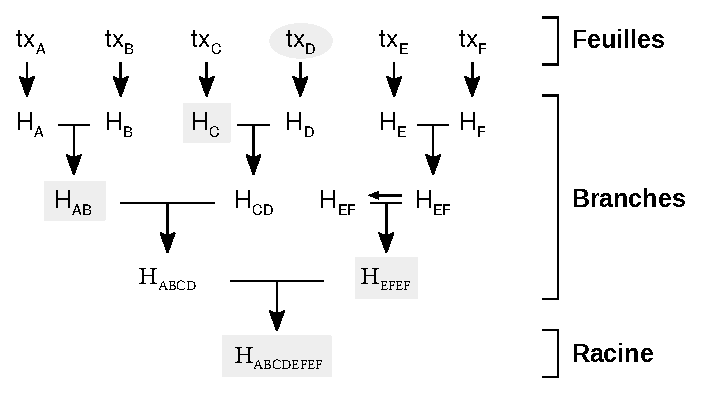
\includegraphics[scale=0.8]{img/merkle-tree.eps}
  \caption{Représentation d'un arbre de Merkle à six feuilles.}
  \label{fig:merkle-tree}
\end{figure}

% Vérification de paiement simplifiée
Cette organisation se révèle particulièrement utile pour les portefeuilles légers (dits à vérification de paiement simplifiée ou SPV) qui ne conservent pas la chaîne de blocs entière mais uniquement la chaîne des entêtes, qui est bien moins volumineuse (un peu plus de 62 Mio en novembre 2023). En effet, pour s'assurer de la présence d'une transaction dans un bloc, ils peuvent se contenter de demander les informations liées à la branche (chemin de Merkle) et procéder aux hachages eux-mêmes\sendnote{Démontrer qu'une feuille fait partie d'un arbre de Merkle requiert de calculer un nombre d'empreintes proportionnel au logarithme binaire du nombre de feuilles ($\log_{2}(n)$), et non pas proportionnel au nombre de feuilles $n$. Pour un bloc de 3~000 transactions (moyenne haute sur BTC), cela représente 12 empreintes de 32 octets à obtenir et 12 hachages à effectuer.}. Par exemple, un utilisateur voulant vérifier la confirmation de la transaction $\mathrm{tx}_D$ doit simplement demander les informations $H_C$, $H_{A\!B}$ et $H_{E\!F\!E\!F}$ aux nœuds du réseau et procéder aux différents hachages pour comparer la racine obtenue avec celle contenue dans l'entête. Cela a pour effet de réduire considérablement la charge des portefeuilles légers.

% Racine de Merkle supplémentaire
Depuis l'activation de SegWit le 24 août 2017, chaque bloc contient un arbre de Merkle supplémentaire, subordonné à l'arbre classique des transactions décrit plus haut. Il s'agit de l'arbre témoin qui est l'arbre des transactions intégrant les signatures des transactions SegWit (séparées des transactions classiques). La racine de l'arbre témoin est placée dans la transaction de récompense, de sorte qu'elle est prise en compte dans la racine de Merkle principale, ce qui garantit l'intégrité de l'ensemble.

% --- Horodatage ---

\subsection{L'horodatage} L'horodatage indique la date et l'heure de construction du bloc qui sont déclarées par le mineur. D'un point de vue technique, il est donné par l'heure Unix, c'est-à-dire le nombre de secondes écoulées depuis le 1\ier{} janvier 1970 \wtime{00:00:00 UTC}. Pour notre bloc, l'horodatage est de $1661407005$ ce qui correspond à la date du 25 août 2022 à 5 heures 56 minutes et 45 secondes (UTC).

\clearpage
Le mineur ne peut pas choisir cet horodatage au hasard. L'heure déclarée doit se situer dans le futur par rapport au temps médian passé (MTP) -- la médiane des horodatages des 11 derniers blocs, qui retarde généralement d'une heure sur le temps réel -- et ne doit pas dépasser l'horloge des nœuds récepteurs de deux heures\pagenote{«~ne doit pas dépasser l'horloge des nœuds récepteurs de deux heures~»~: \url{https://github.com/bitcoin/bitcoin/blob/24.x/src/validation.cpp\#L3483-L3490}.}. Cette contrainte relativement permissive permet au temps réseau de rester relativement cohérent avec la réalité.

% --- Valeur cible ---

\subsection{La valeur cible} La valeur cible est la valeur minimale que l'identifiant du bloc peut prendre pour que ce bloc constitue une preuve de travail. Plus cette valeur cible est petite, plus il est facile de trouver une solution et de miner un bloc. Elle est déterminée par le réseau selon les règles de l'algorithme d'ajustement de la difficulté.

La valeur cible est encodée comme un nombre flottant où le premier octet représente un exposant particulier et où la mantisse est déterminée par les 3 octets suivants. Ici, elle est égale à $\mathtt{0x09ed88} \times 256^{(\mathtt{0x17} - 3)}$ c'est-à-dire~:

\begin{Verbatim}[fontsize=\footnotesize]
00000000000000000009ed880000000000000000000000000000000000000000
\end{Verbatim}

Cette information donne aussi la difficulté de minage du bloc, qui est inversement proportionnelle à la valeur cible. Il s'agit du quotient de la valeur cible maximale du système par la valeur cible du réseau\sendnote{En notant $c$ la valeur cible, la difficulté est définie par~: \[ d = \frac{C_{\mathrm{max}}}{c} \] où $C_{\mathrm{max}} = \mathtt{0x00ffff} \times 256^{26}$ est la valeur cible maximale du réseau.}. La difficulté minimale du protocole est donc de 1 et celle de notre bloc (arrondie à l'unité près) est quant à elle de $28~351~606~743~494$, ce qui représente un différentiel énorme~! Elle donne également la quantité de travail du bloc, qui est le nombre moyen de hachages nécessaires pour tomber sur une solution\sendnote{En termes mathématiques, le travail d'un bloc est le quotient du nombre d'empreintes possibles par le nombre d'empreintes satisfaisant le problème. En notant $c$ la valeur cible, le travail est~: \[ T = \frac{2^{256}}{c + 1} ~.\]}.

% --- Nonce ---

\subsection{Le nonce} Le nonce désigne le nombre que le mineur fait varier pour produire la preuve de travail. Ce mot provient de l'expression anglaise «~\eng{for the nonce}~» signifiant «~pour la circonstance, pour l'occasion~», ce qui indique la spécificité de son rôle\sendnote{Une étymologie populaire prétend qu'il serait une contraction de l'expression «~\eng{number used once}~», mais celle-ci est incorrecte.}. Le mineur fait également varier un nonce supplémentaire au sein de la transaction de récompense, le champ du nonce étant trop petit (8 octets) pour la difficulté de minage actuelle. Le nonce de notre bloc est $4~224~551~499$.

Ces deux derniers paramètres (valeur cible et nonce) sont relatifs à la preuve de travail et interviennent dans la formulation du problème mathématique résolu par le mineur. Ce problème se présente sous la forme d'une inégalité mathématique. En notant $c$ la valeur cible du réseau et $\mathrm{EB}$ l'entête du bloc, il s'agit de trouver un nonce $n$ tel que~:

{ \footnotesize
\[
\mathrm{SHA256d} ( \ \mathrm{EB} ( \ n \ ) \ ) ~ \le ~ c
\]
}

Comme on l'a dit, le résultat est utilisé comme identifiant du bloc. La preuve de travail est facilement vérifiable~: chaque membre du réseau peut, à partir des données du bloc, s'assurer que le mineur a bien trouvé une solution valide. Dans notre cas, si on compare l'identifiant et la valeur cible, on obtient bien un résultat qui satisfait l'inégalité exigée~:

{ \footnotesize
\begin{align*}
\mathtt{0x000000000000000000065aebf106c8824f4b565d54d6d6df32498b2b041cfd07} & \le \\ \mathtt{0x00000000000000000009ed880000000000000000000000000000000000000000} & ~
\end{align*}
}

\begin{figure}[h]
  \centering
  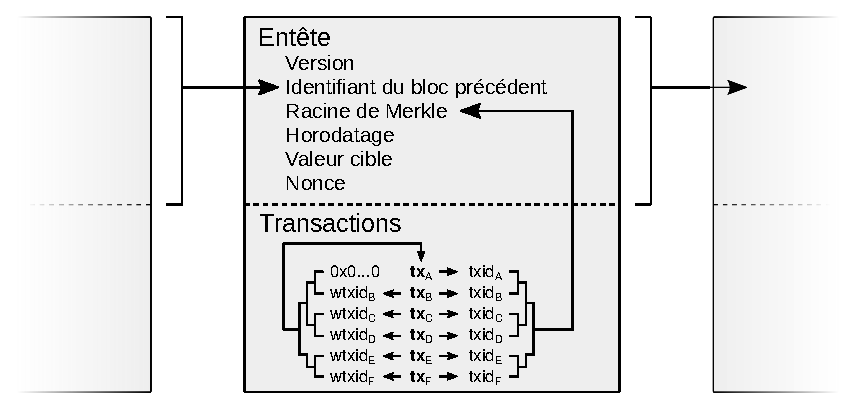
\includegraphics[scale=0.75]{img/bitcoin-segwit-block.eps}
  \caption{Schéma d'un bloc de Bitcoin (avec SegWit).}
  \label{fig:bitcoin-segwit-block}
\end{figure}

\section*{Le revenu du minage} % Le minage, un procédé économique
\addcontentsline{toc}{section}{Le revenu du minage}

% --- Présentation du minage ---

L'une des innovations de Bitcoin est de récompenser la confirmation des transactions à l'aide de son unité de compte interne. Cette propriété crée une incitation économique poussant les mineurs à bien se comporter, ce qui contribue à la solidité du système.

La récompense liée à l'ajout d'un bloc à la chaîne provient en partie de la création monétaire du protocole, d'où le nom de minage employé pour désigner cette activité. Le procédé est en effet analogue à l'extraction minière de l'or dans le monde réel~: les mineurs déploient du capital et dépensent de l'énergie pour obtenir les nouveaux bitcoins. Comme expliqué par Satoshi dans le livre blanc~:

\begin{quote}
«~L'ajout régulier d'une quantité constante de nouvelles pièces est analogue aux mineurs d'or qui dépensent des ressources pour ajouter de l'or à la circulation\sendnote{Satoshi Nakamoto, \eng{Bitcoin: A Peer-to-Peer Electronic Cash System}, 31 octobre 2008.}.~»
\end{quote}

La deuxième partie de la récompense provient des frais de transaction payés par les utilisateurs, qui sont collectés sur les transactions incluses dans le bloc. Le tout est reversé au mineur lorsque le bloc est vérifié et accepté par le réseau. % Le tout est reversé au mineurs lors de la publication d'un bloc valide accepté par le réseau.

% Définition du minage
Le minage est ainsi l'activité économique consistant à rassembler les transactions au sein d'un bloc, à produire la preuve de travail et à diffuser le résultat sur le réseau. Ici, nous le distinguons ainsi du simple hachage, qui consiste juste à réaliser les calculs pour créer la preuve de travail et qui peut être réalisé indépendamment de la sélection de transactions, notamment au sein des coopératives de minage (\eng{mining pools}). Dans ce cadre, les mineurs sont les personnes ou les groupes de personnes réalisant l'activité complète, et les entités se contentant de mettre en place des machines et de déléguer leur pouvoir sur la sélection des transactions ne sont que des «~hacheurs~».

% L'entité réalisant cette activité est appelée un mineur\sendnote{Le terme de mineur peut également parfois désigner la machine utilisée pour produire la preuve de travail.}.

% Déroulement du minage d'un bloc
Le minage se déroule de manière cyclique. Tout d'abord, le mineur sélectionne des transactions à partir de la réserve des transactions (appelée \eng{mempool}) de son nœud. Puis, il construit un bloc candidat en imposant un entête, en assemblant les transactions et en prenant soin de construire une transaction de récompense qui le rémunère. Il fait ensuite varier le nonce et d'autres éléments du bloc candidat afin de produire la preuve de travail. Enfin, dans le cas où il trouve une solution, il diffuse le bloc sur le réseau le plus rapidement possible pour que les autres nœuds le vérifient et l'acceptent comme le nouveau bloc de la chaîne. Dans le cas contraire, si un nouveau bloc est trouvé entretemps, le mineur l'accepte et abandonne son bloc candidat. Dans les deux cas, la procédure reprend du début avec des transactions différentes.

% Transaction de récompense (coinbase)
La récompense de minage est ainsi récupérée par le mineur via l'inclusion d'une transaction de récompense au sein du bloc. Celle-ci doit être, par convention, la première transaction du bloc. Elle possède une entrée unique spécifique ne faisant référence à aucune transaction existante. La transaction de récompense est aussi appelée la base de pièce ou \eng{coinbase}, car c'est à partir d'elle que sont formés les nouveaux bitcoins. Le mineur dirige cette transaction vers une adresse qu'il contrôle, de sorte qu'il est récompensé si et seulement si son bloc est valide aux yeux du réseau. La récompense que le mineur peut se verser doit être inférieure à la somme de la création monétaire et des frais de transaction. Le mineur peut ainsi se rémunérer moins que ce qui est prévu par le protocole, même si cela n'a aucun sens économique direct\sendnote{En décembre 2017, le mineur du bloc 501~726 s'est ainsi rémunéré de la coquette somme de 0~BTC~!}.

% --- Création monétaire ---

La création monétaire se fait intégralement par le biais de la transaction de récompense. Tous les bitcoins dans le système sont ainsi le résultat d'une série de transferts commençant par une telle transaction.

% La particularité de Bitcoin par rapport à ses prédécesseurs, et notamment le système RPOW, est d'offrir une politique monétaire fixe malgré un recours à la preuve de travail. Cette caractéristique permet d'éviter la création monétaire liée à l'innovation technique, qui est exponentielle comme l'illustre la loi de Moore.

% Ajustement de la difficulté
La particularité de cette création monétaire est qu'elle est fixée dans le temps et qu'elle n'est pas proportionnelle à la puissance de calcul déployée. Cela est rendu possible par l'algorithme d'ajustement de la difficulté, qui dérive du fait que le système constitue un serveur d'horodatage distribué. En effet, les blocs étant horodatés, il est possible de mesurer leur rythme de production passé et d'ajuster la difficulté de minage en conséquence. Ainsi, comme l'écrivait Satoshi~:

\begin{quote}
«~Afin de compenser l'augmentation de la vitesse du matériel et la variation de l'intérêt des nœuds actifs au fil du temps, la difficulté de la preuve de travail est déterminée par une moyenne mobile visant un nombre moyen de blocs par heure. Si ces blocs sont générés trop rapidement, la difficulté augmente\sendnote{Satoshi Nakamoto, \eng{Bitcoin: A Peer-to-Peer Electronic Cash System}, 31 octobre 2008.}.~»
\end{quote}

Dans la version principale de Bitcoin, l'intervalle de temps entre chaque bloc (temps de bloc) visé est de 10 minutes ou 600 secondes. L'ajustement a lieu tous les 2016 blocs, ce qui correspond environ à deux semaines, selon la moyenne simple du temps de bloc sur cette période. La nouvelle valeur cible est calculée\sendnote{Dans Bitcoin Core, l'algorithme d'ajustement est décrit par la fonction \longstring{CalculateNextWorkRequired} dans le fichier \texttt{pow.cpp}. La variation est limitée à un facteur 4 (multiplication comme division) pour éviter les instabilités. L'algorithme \emph{surestime} la puissance de calcul déployée car le temps écoulé est mesuré sur 2~015 intervalles, et non pas 2~016 comme cela devrait se faire.}\pagenote{«~la fonction CalculateNextWorkRequired dans le fichier pow.cpp~»~: \url{https://github.com/bitcoin/bitcoin/blob/24.x/src/pow.cpp\#L49-L72}.} à partir de la valeur cible précédente ($c_{k-1}$) et du temps écoulé depuis le dernier ajustement ($t_{k-1}$)~:

{ \footnotesize
\[
c_{k} = \frac{c_{k-1} \cdot t_{k-1}}{2016 \cdot 600}
\]
}

% Politique monétaire
Grâce à cet ajustement, le bitcoin possède une politique monétaire déterminée, qui n'est pas soumise à l'arbitraire direct d'un tiers de confiance ou à la quantité de capital déployé. Cette caractéristique le différencie de la monnaie fiat (comme le dollar) qui est émise de manière discrétionnaire par une banque centrale, ou du métal précieux (comme l'or) dont la quantité extraite connaît ses propres variations et suit la demande du marché à long terme. Cette politique monétaire a été décrite précisément pour la première fois par Satoshi Nakamoto dans son courriel de lancement du 8 janvier 2009 où il écrivait~:

\begin{quote}
«~La quantité en circulation totale sera de 21~000~000 pièces. Elle sera distribuée aux nœuds du réseau lorsqu'ils créeront des blocs, le montant étant divisé par deux tous les 4 ans.

les quatre premières années : 10~500~000 pièces\\
les quatre années suivantes : 5~250~000 pièces\\
les quatre années suivantes : 2~625~000 pièces\\
les quatre années suivantes : 1~312~500 pièces\\
etc...

Lorsque cela est épuisé, le système peut prendre en charge les frais de transaction si nécessaire. Il est basé sur la concurrence du marché ouvert, et il y aura probablement toujours des nœuds prêts à traiter les transactions gratuitement\sendnote{Satoshi Nakamoto, \eng{Bitcoin v0.1 released}, \wtime{08/01/2009 19:27:40 UTC}~: \url{https://www.metzdowd.com/pipermail/cryptography/2009-January/014994.html}.}.~»
\end{quote}

Elle est bien évidemment inscrite dans le code\pagenote{«~Elle est bien évidemment inscrite dans le code~»~: \url{https://github.com/bitcoin/bitcoin/blob/24.x/src/validation.cpp\#L1473-L1484}}, où elle est appelée subvention ou \eng{subsidy} en anglais.

% Réduction de moitié
L'originalité principale de cette politique monétaire est que la création monétaire est réduite de moitié de manière brusque tous les 210~000 blocs (soit environ 4 ans) lors de ce qu'on appelle couramment un \eng{halving}. En 2023, trois réductions de moitié avaient déjà eu lieu sur le réseau Bitcoin principal~: la première s'est produite le 28 novembre 2012, lorsque la subvention du protocole est passée de 50 bitcoins par bloc à 25~; la deuxième le 9 juillet 2016, avec une baisse à 12,5 bitcoins par bloc~; la troisième le 11 mai 2020, où la subvention a été réduite à 6,25 bitcoins par bloc. La prochaine réduction de moitié devrait se passer en avril 2024, après laquelle les nouveaux bitcoin émis seront de 3,125 par bloc. Sauf modification des règles de consensus, la dernière réduction de moitié sera la 33\ieme{} et aura lieu aux alentours de 2140. En effet, le montant de création monétaire par bloc passera alors en dessous du satoshi, soit zéro par troncature à l'unité.

% old function:
%
% \begin{Verbatim}[fontsize=\footnotesize]
% int64 CBlock::GetBlockValue(int64 nFees) const
% {
%     int64 nSubsidy = 50 * COIN;
% 
%     // Subsidy is cut in half every 4 years
%     nSubsidy >>= (nBestHeight / 210000);
% 
%     return nSubsidy + nFees;
% }
% \end{Verbatim}


% Limite des 21 millions
À long terme, cette politique monétaire atypique fait du bitcoin une monnaie à quantité fixe. En effet, le montant maximal de bitcoins en circulation doit tendre, au fil du temps, vers une limite~: la fameuse limite des 21 millions. Celle-ci n'est qu'une déduction des conditions d'émission susmentionnées, ce qui s'exprime en termes mathématiques par la convergence de la série des montants minés entre les halvings\sendnote{Cette convergence est illustrée par le paradoxe d'Achille et de la tortue formulé par le philosophe grec Zénon. La suite $\left( \sum_{i=1}^{n} (1/2)^i \right)$ converge vers $1$ lorsque $n\to+\infty$.}~:

{ \footnotesize
\[
N_{\mathrm{max}} = \sum_{i=0}^{+\infty} \left( {210~000 \cdot \frac{50}{2^i}} \right) = 21~000~000 \cdot \sum_{i=1}^{+\infty} \left(\frac{1}{2}\right)^i = 21~000~000
\]
}

% Limite jamais atteinte
La limite des 21 millions est une borne supérieure~: en l'absence d'un changement des règles de consensus, elle ne sera jamais formellement atteinte, en raison de la nature optionnelle de la récompense de minage, du caractère discret des unités et de la perte irrémédiable de bitcoins. De plus, les bitcoins dont les propriétaires ont perdu leurs clés privées réduisent considérablement la quantité réelle de bitcoins en circulation sans pour autant que cela ne soit pris en compte dans le calcul.

% Remplacement par les frais
La création monétaire a ainsi vocation à s'amenuiser et à devenir négligeable, et ce plus rapidement que l'on imagine. En effet, en 2023, le nombre de bitcoins dépensables avait déjà dépassé les 19,5 millions. C'est pourquoi cette subvention doit en toute logique être remplacée par l'autre source de revenu pour les mineurs, à savoir les frais de transaction\sendnote{«~Une fois qu'un nombre prédéterminé de pièces a été mis en circulation, l'incitation peut être entièrement financée par les frais de transaction et ne plus requérir aucune inflation.~» -- Satoshi Nakamoto, \eng{Bitcoin: A Peer-to-Peer Electronic Cash System}, 24 mars 2009.}.

% Frais de transaction
Les frais de transaction sont les commissions payées par les utilisateurs pour la confirmation de leurs transactions. Les frais d'une transaction peuvent être versés directement par l'expéditeur (client) ou indirectement par le destinataire (commerçant) par l'intermédiaire d'une remise sur le produit vendu. Ils sont récupérés par le mineur sur chaque transaction du bloc selon une règle implicite~: il s'agit de la différence entre le montant en entrée de la transaction et son montant en sortie. Cette différence peut être de zéro (transaction gratuite), mais elle est toujours comptabilisée. Les frais sont ajoutés à la transaction de récompense indistinctement des bitcoins issus de la création monétaire. Bitcoin intègre ainsi un système interne et optimisé de frais de transaction, qui évite l'alourdissement inutile des transactions et des blocs.

% Existence des frais
L'existence des frais de transaction a vocation à perdurer par conception, même si ceux-ci devenaient très bas. Contrairement à l'opinion exprimée par Satoshi, la confirmation d'une transaction a en général un coût, même marginal\sendnote{Le seul cas envisageable de transaction gratuite est celui d'une grande transaction de consolidation qui amoindrirait la charge des mineurs en réduisant considérablement l'ensemble des sorties transactionnelles non dépensées.}, et une transaction qui paie trop peu de frais par rapport à la charge apportée n'a aucune raison économique d'être confirmée. De ce fait, il n'y a pas lieu de s'imaginer que la chaîne de blocs s'arrête.

% Limite de capacité transactionnelle
En outre, les règles du protocole restreignent usuellement l'espace de bloc par le biais d'une limite explicite sur la taille (ou le poids) des blocs. Cette restriction crée un plafond de production qui, lorsqu'il est atteint, fait que le mineur rationnel sélectionne les transactions qui paient le taux le plus élevé de frais, toutes choses étant égales par ailleurs. Il existe donc, dans le cas d'une congestion du réseau, un effet d'enchères pouvant faire augmenter le niveau moyen des frais de manière drastique.

% --- Alternatives aux frais ---

Bien que les frais constituent la façon principalement envisagée de rémunérer les mineurs à terme, des méthodes alternatives de financement ont été proposées.

% Émission résiduelle
La première est l'émission résiduelle (\eng{tail emission}), qui consiste à maintenir une création monétaire constante au cours du temps, dans le but que le revenu de minage ne tombe pas trop bas\sendnote{Peter Todd, \eng{Surprisingly, Tail Emission Is Not Inflationary}, 9 juillet 2022~: \url{https://petertodd.org/2022/surprisingly-tail-emission-is-not-inflationary}.}. L'instauration de cette caractéristique aurait pour effet de modifier la politique monétaire du bitcoin et de faire disparaître la limite des 21 millions, d'où son caractère hautement controversé.

Pour donner un exemple, l'émission résiduelle est mise en place dans la variante Monero depuis 2015. Elle est devenue effective le 9 juin 2022, date depuis laquelle il se crée 0,3~monero par minute, soit un taux de création monétaire annualisé de 0,87~\% à ce moment-là. Une telle émission résiduelle existe également dans Dogecoin depuis 2015, à raison de 10~000 dogecoins par minute, pour un taux annualisé de 3,7~\% en novembre 2023.

% Demeurage
La deuxième méthode de financement proposée est le demeurage, ou coût de détention, qui consiste à prélever la monnaie demeurée immobile depuis un temps donné\sendnote{Jorge Timón, \eng{Freicoin: bitcoin with demurrage}, \wtime{24/02/2011 11:56:03 UTC}~: \url{https://bitcointalk.org/index.php?topic=3816.msg54170\#msg54170}.}. Les bitcoins de Satoshi, qui représentent une manne financière importante, sont notamment concernés. Toutefois, il s'agirait d'une atteinte au système de propriété de Bitcoin et il y a donc peu de chances que cette méthode rencontre le succès.

\section*{La chaîne la plus longue}
\addcontentsline{toc}{section}{La chaîne la plus longue}

Venons-en maintenant au sujet central de ce chapitre~: l'atteinte du consensus par le minage. Comme nous l'avons expliqué ci-dessus, le minage est le procédé permettant aux mineurs d'ajouter des blocs à la chaîne, chose pour laquelle ils sont rémunérés. Mais nous n'avons pas exposé comment il permettait d'arriver à un accord dans un contexte antagoniste, en présence d'acteurs malveillants «~byzantins~».

% Communication
Les nœuds suivent un protocole composé des règles de réseau, qui leur permettent de rentrer en communication, et des règles de consensus, qui concernent la forme des transactions et des blocs, que nous détaillerons dans le chapitre~\ref{ch:changement}. Les nœuds qui enfreignent ces règles voient leurs connexions être fermées par leurs pairs et sont mis sur liste noire si nécessaire. Il est donc impossible de faire accepter une transaction ou un bloc au réseau qui ne soit valide selon les règles de consensus.

Néanmoins, les nœuds byzantins peuvent semer la discorde dans le respect des règles de consensus, en produisant des blocs concurrents. En effet, rien n'empêche \emph{a priori} un attaquant de produire des blocs de transactions qui soient valides mais qui ne soient pas rattachés à la branche principale et de les soumettre au réseau.

% --- Principe de la chaîne la plus longue ---

Ce problème est résolu par le biais d'un principe simple mais efficace~: le principe de la chaîne la plus longue. Celui-ci a été décrit par Satoshi dans le livre blanc~: 

\begin{quote}
«~La décision majoritaire est représentée par la chaîne la plus longue, sur laquelle le plus grand effort de preuve de travail a été investi\sendnote{Satoshi Nakamoto, \eng{Bitcoin: A Peer-to-Peer Electronic Cash System}, 31 octobre 2008.}.~»
\end{quote}

Les nœuds du réseau se mettent d'accord en sélectionnant la chaîne possédant le plus de travail accumulé\pagenote{«~la chaîne possédant le plus de travail accumulé~»~: Ce principe a été redéfini le 25 juillet 2010 au sein de la version 0.3.3 du logiciel~: \url{https://github.com/bitcoin/bitcoin/commit/3b7cd5d89a226426df9c723d1f9ddfe08b7d1def}.}, ce qui se matérialise généralement par une chaîne plus longue en nombre de blocs\sendnote{En réalité, au début c'était bel et bien la chaîne possédant le plus de blocs qui était sélectionnée. Mais ce principe a été redéfini le 25 juillet 2010 au sein de la version 0.3.3 du logiciel pour prendre en compte la notion de travail.}. Lorsqu'une chaîne possédant une quantité strictement plus grande de travail est publiée, les nœuds suivent cette chaîne, que celle-ci soit dans la continuité de la dernière ou qu'elle fasse référence à une branche plus ancienne. Cette règle fait en sorte que les nœuds suivent toujours la chaîne sur laquelle un montant supérieur d'énergie a été investi. L'algorithme de consensus résultant de l'application de ce principe est appelé l'algorithme de consensus de Nakamoto par preuve de travail, en hommage à son concepteur.

% --- Embranchement ---

La meilleure manière d'appréhender le fonctionnement de cet algorithme est de prendre le cas d'un embranchement (appelé \eng{fork} en anglais) de la chaîne. Celui-ci peut être créé par un acteur malveillant, mais dans la réalité il est généralement engendré de manière accidentelle, lorsque deux mineurs éloignés trouvent chacun un bloc différent dans un intervalle de temps réduit et que les nœuds du réseau ne reçoivent pas le même bloc en premier. Il n'y a alors aucun moyen de départager les deux branches, celles-ci étant également correctes en vertu du principe de la chaîne la plus longue. Ce type d'embranchement accidentel est commun et se produit de temps en temps sur le réseau pour des raisons de latence.

Cette situation et sa résolution ont été décrites par Satoshi dans le livre blanc~:

\begin{quote}
«~Si deux nœuds transmettent simultanément des versions différentes du bloc suivant, certains nœuds peuvent recevoir l'une ou l'autre version en premier. Dans ce cas, ils travaillent sur la première version qu'ils ont reçue, mais conservent l'autre branche au cas où elle deviendrait plus longue. L'égalité est rompue lorsque la preuve de travail suivante est trouvée et qu'une branche devient plus longue~; les nœuds qui travaillaient sur l'autre branche passent alors sur la chaîne la plus longue\sendnote{Satoshi Nakamoto, \eng{Bitcoin: A Peer-to-Peer Electronic Cash System}, 31 octobre 2008.}.~»
\end{quote}

Le réseau passe par trois étapes. Tout d'abord, il se comporte de manière attendue~: les mineurs prolongent la chaîne la plus longue, sur laquelle le reste des nœuds se coordonnent. Puis, le conflit a lieu~: deux branches correctes coexistent et les mineurs travaillent pour prolonger la chaîne à partir du bloc reçu en premier. Enfin, l'embranchement est résolu~: un mineur trouve un nouveau bloc et sa chaîne, qui devient plus longue, est acceptée par le réseau.

Il se produit alors ce qu'on appelle une recoordination (\eng{reorganization}) qui réconcilie les nœuds du réseau entre eux. Le bloc de la branche faible est considéré comme incorrect et mis de côté. On dit que ce bloc est rendu orphelin (\eng{orphaned}) car il perd son attachement à la chaîne mère\sendnote{L'appellation (quelque peu ambigüe) de «~bloc orphelin~» a été introduite par Satoshi Nakamoto au sein de la première version du logiciel. On parle aussi de «~bloc oncle~» (en référence au fait qu'il ne donne pas de descendance fertile) ou bien de «~bloc périmé~» (\eng{stale block}).}. La branche forte (possédant le plus de travail accumulé) est considérée comme la version correcte de la chaîne.

\begin{figure}[h]
  \centering
  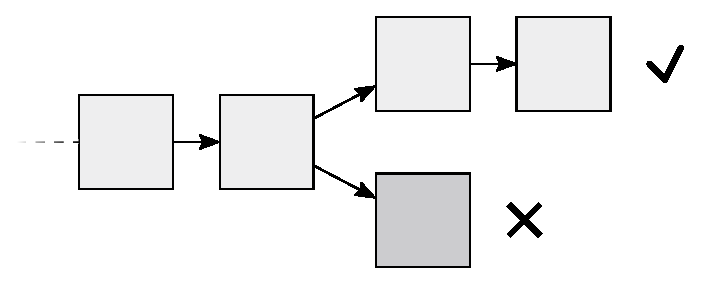
\includegraphics[scale=0.8]{img/blockchain-common-fork.eps}
  \caption{Schéma d'un embranchement commun de la chaîne.}
  \label{fig:blockchain-common-fork}
\end{figure}

Tout conflit sur le réseau est résolu de la sorte, ce qui a pour conséquence de conférer une nature particulière à l'algorithme de Nakamoto, et par extension à Bitcoin.

% Tout conflit sur le consensus est résolu de la sorte. Le fonctionnement de l'algorithme de Nakamoto possède des conséquences sur la nature de Bitcoin.

% --- Deux contraintes sécuritaires ---

% Honnêteté de la majorité
Ce fonctionnement impose tout d'abord deux contraintes majeures sur la sécurité. La première est que la sécurité minière du réseau repose sur la supposition qu'une majorité de la puissance de calcul («~51~\%~») se comporte de manière honnête. Comme l'expliquait Satoshi~:

\begin{quote}
«~Le système est sécurisé tant que les nœuds honnêtes contrôlent collectivement plus de puissance de calcul qu'un groupe de nœuds qui coopéreraient pour réaliser une attaque\sendnote{Satoshi Nakamoto, \eng{Bitcoin: A Peer-to-Peer Electronic Cash System}, 31 octobre 2008.}.~»
\end{quote}

% Sécurité probabiliste
La seconde est que la sécurité d'une transaction donnée est probabiliste et dépend de la profondeur à laquelle elle se trouve dans la chaîne. La transaction est d'abord vérifiée par le réseau (zéro confirmation), puis confirmée au sein d'un bloc (une confirmation) et finit par être considérée comme irréversible, généralement à partir de six confirmations pour les montants ordinaires sur la version principale de Bitcoin. Cela contraint l'utilisateur à estimer le nombre de confirmations qu'il doit attendre en fonction de la sécurité désirée.

% Période de maturation de la récompense de minage
Cette particularité se transcrit dans le fonctionnement du minage par la maturité de la base de pièce (\eng{coinbase maturity}), qui est le nombre de confirmations nécessaire pour que la sortie de la transaction de récompense devienne dépensable. Cette contrainte est mise en place pour éviter la mauvaise utilisation des fonds due à une recoordination peu profonde. Le délai sur le réseau BTC est aujourd'hui de 101 confirmations\pagenote{«~Le délai sur le réseau BTC est aujourd'hui de 101 confirmations~»~: \url{https://github.com/bitcoin/bitcoin/blob/23.x/src/consensus/consensus.h\#L18-L19}}.

% --- Trois avantages ---

% Objectivité
L'algorithme de Nakamoto possède également trois avantages principaux. D'abord, il a pour intérêt d'avoir un critère objectif sur lequel se reposer~: tout le monde peut reconstituer la chaîne à partir du bloc de genèse et constater qu'il s'agit de la chaîne correcte. Même dans le cas extrême d'un cloisonnement mondial et prolongé du réseau dû à une guerre ou une catastrophe naturelle, le système peut finir par se recoordonner\sendnote{Satoshi Nakamoto, \eng{Re: Anonymity}, \wtime{08/07/2010, 19:12:00 UTC}~: \url{https://bitcointalk.org/index.php?topic=241.msg2071\#msg2071}.}.

% Ouverture
Ensuite, il permet la participation ouverte au consensus~: tout ce qui est requis du mineur est une preuve de travail valide, de sorte que le minage est anonyme par essence.

% Robustesse
Enfin, cet algorithme par preuve de travail assure la robustesse du réseau~: un mineur n'a pas à connaître tous les autres participants, ce qui permet au réseau d'être composé de dizaines (voire de centaines) de milliers de nœuds.

\vspace{-1em}
\section*{La résistance à la double dépense}
\addcontentsline{toc}{section}{La résistance à la double dépense}

La double dépense est le fait pour un acteur de faire accepter successivement deux transactions au réseau dans le but de déstabiliser l'état du système et d'en bénéficier d'une manière ou d'une autre. La deuxième transaction peut constituer une annulation de la première, dans laquelle l'acteur malveillant réalise un transfert vers lui-même.

% Transactions non confirmées
La double dépense constitue un problème dans le cas des transactions non confirmées, c'est-à-dire des transactions qui ont été diffusées sur le réseau, vérifiées par les nœuds et placées dans leurs \eng{mempools}, mais qui n'ont pas encore été incluses dans un bloc de la chaîne. Aucun consensus n'a été réalisé à propos de ces transactions, mais le commerçant peut décider de les accepter dans le cas où les montants engagés sont faibles\sendnote{Dans un message sur le forum en juillet 2010, Satoshi écrivait à propos de l'acceptation des transactions non confirmées~: «~Je pense qu'il sera possible pour une entreprise de traitement des paiements de fournir comme service la distribution rapide de transactions avec une vérification suffisante en 10 secondes ou moins. Les nœuds du réseau n'acceptent que la première version d'une transaction qu'ils reçoivent pour l'incorporer dans le bloc qu'ils essaient de générer. Lorsqu'on diffuse une transaction et que quelqu'un d'autre diffuse une double dépense au même moment, c'est une course à la propagation vers le plus grand nombre de nœuds qui a lieu. Si l'une d'elles a une légère avance, elle se propagera géométriquement dans le réseau plus rapidement et atteindra la plupart des nœuds. [...] Le processeur de paiement a des connexions avec de nombreux nœuds. Lorsqu'il reçoit une transaction, il l'envoie et, en même temps, surveille le réseau pour détecter les doubles dépenses. S'il reçoit une double dépense sur l'un de ses nombreux nœuds d'écoute, il signale que la transaction est mauvaise.~» -- Satoshi Nakamoto, \eng{Re: Bitcoin snack machine (fast transaction problem)}, \wtime{17/07/2010 22:29:13 UTC}~: \url{https://bitcointalk.org/index.php?topic=423.msg3819\#msg3819}.}. Le risque est qu'un fraudeur reparte avec la marchandise et réussisse à faire accepter une version alternative de la transaction vue par le commerçant, soit en la diffusant au même moment et en espérant qu'elle arrive en premier au mineur, soit en payant plus de frais (ce qui peut être fait systématiquement avec Replace-by-Fee) pour soudoyer le mineur, soit encore en minant préalablement un bloc contenant la transaction (attaque Finney\sendnote{Hal Finney, \eng{Re: Best practice for fast transaction acceptance - how high is the risk?}, \wtime{13/02/2011, 21:48:44 UTC}~: \url{https://bitcointalk.org/index.php?topic=3441.msg48384\#msg48384}.}).

% Solution : le minage
La solution à ce problème est de se mettre d'accord sur la transaction correcte pour faire disparaître la double dépense, \emph{ce qui est précisément le but du minage}. Cependant, le minage n'empêche pas la double dépense de manière absolue, étant plutôt un mécanisme de résistance. Voyons ce qui garantit cette caractéristique.

% --- Attaque de double dépense par recoordination de chaîne ---

Un certain nombre de perturbations opportunistes peuvent avoir lieu au niveau de l'activité minière comme l'attaque vector76\sendnote{vector76, \eng{Re: Fake Bitcoins?}, \wtime{17/08/2011 17:37:56 UTC}~: \url{https://bitcointalk.org/index.php?topic=36788.msg463391\#msg463391}.} ou le minage égoïste\sendnote{Ittay Eyal, Emin Gün Sirer, \eng{Majority is not Enough: Bitcoin Mining is Vulnerable}, 2013.}, mais la plus importante d'entre elles est l'attaque de double dépense par recoordination de chaîne. Celle-ci consiste à utiliser une part importante de la puissance de calcul du réseau (généralement une majorité) afin de réécrire le passé de la chaîne et modifier une ou plusieurs transactions. Cette attaque a été décrite précisément par Satoshi Nakamoto dans le livre blanc\sendnote{«~Nous considérons le scénario d'un attaquant qui tente de générer une chaîne alternative plus rapidement que la chaîne honnête. Même en cas de réussite, cela n'expose pas le système à des modifications arbitraires [...]. Un attaquant peut seulement essayer de modifier l'une de ses propres transactions afin de récupérer l'argent qu'il a récemment dépensé.~» -- Satoshi Nakamoto, \eng{Bitcoin: A Peer-to-Peer Electronic Cash System}, 31 octobre 2008.} et dans son courriel de réponse à John Levine du 3 novembre 2008\sendnote{«~Même si un individu malintentionné parvenait à maîtriser le réseau, ce n'est pas comme s'il devenait instantanément riche. Tout ce qu'il pourrait faire, c'est récupérer l'argent qu'il a lui-même dépensé, comme un chèque sans provision. Pour l'exploiter, il faudrait qu'il achète une chose à un commerçant, qu'il attende qu'elle soit expédiée, puis qu'il prenne le contrôle du réseau et essaie de récupérer son argent. Je ne pense pas qu'il puisse se faire autant d'argent en essayant de monter un tel stratagème qu'en générant des bitcoins. Avec une ferme de machines zombies aussi grande, il pourrait générer plus de bitcoins que tous les autres réunis.~» -- Satoshi Nakamoto, \eng{Re: Bitcoin P2P e-cash paper}, \wtime{03/11/2008 16:23:49}~: \url{https://www.metzdowd.com/pipermail/cryptography/2008-November/014818.html}.}. % "Even if a bad guy does overpower the network, it's not like he's instantly rich.  All he can accomplish is to take back money he himself spent, like bouncing a check.  To exploit it, he would have to buy something from a merchant, wait till it ships, then overpower the network and try to take his money back.  I don't think he could make as much money trying to pull a carding scheme like that as he could by generating bitcoins.  With a zombie farm that big, he could generate more bitcoins than everyone else combined."

% Majorité de la puissance de calcul
Cette attaque est réalisée en trois étapes. Elle peut être faite à l'aide d'une minorité de la puissance de calcul, auquel cas elle ne possède qu'une certaine probabilité de réussir. Cependant, par souci de simplicité, nous supposerons qu'un mineur a réuni la majorité de la puissance de calcul du réseau. L'attaque constitue donc une attaque des 51~\%, aussi appelée attaque de la majorité.

% Achat d'un bien
La première étape est l'achat d'un bien ou d'un service auprès d'un commerçant. L'attaquant procède à une transaction en bitcoins (dite «~légitime~») en l'échange de quoi le commerçant lui fournit une chose de même valeur. Typiquement, il s'agira d'une autre cryptomonnaie ou du dollar auprès d'une plateforme de change.

% Minage d'une chaîne parallèle
La deuxième étape est le minage d'une chaîne parallèle. Une fois que la transaction légitime a été confirmée au sein d'un bloc, l'attaquant construit une chaîne parallèle en secret à partir du bloc précédent, qu'il prend soin de ne pas dévoiler au reste du réseau. Dans le même temps, il crée et signe une autre transaction (dite «~frauduleuse~») qui dépense les mêmes bitcoins que la première et qui les renvoie vers une adresse en son contrôle. Il inclut cette transaction frauduleuse dans sa chaîne parallèle. Puisque l'attaquant dispose de la majorité de la puissance de calcul du réseau, il est sûr qu'à un moment ou à un autre, cette chaîne sera plus longue que l'autre.

% Recoordination
La troisième étape est la recoordination de chaîne, représentée sur la figure~\ref{fig:doublespending-attack}. L'attaquant a continué de miner sa chaîne parallèle jusqu'à la livraison du bien économique acheté. À ce moment-là, il dévoile sa chaîne au reste du réseau, qui doit accepter celle-ci en vertu du principe de la chaîne la plus longue. Les nœuds procèdent alors à une recoordination~: les blocs de l'ancienne chaîne sont écartés (rendus orphelins), leurs transactions sont remises dans la mempool et les nouveaux blocs sont vérifiés et ajoutés à la chaîne. Comme la transaction légitime dépense les mêmes fonds que la transaction frauduleuse, qui est incluse dans la nouvelle chaîne, cette transaction légitime est invalidée en tant que double dépense. Le commerçant ne possède plus les bitcoins, qui reviennent à l'attaquant.

\begin{figure}[h]
  \centering
  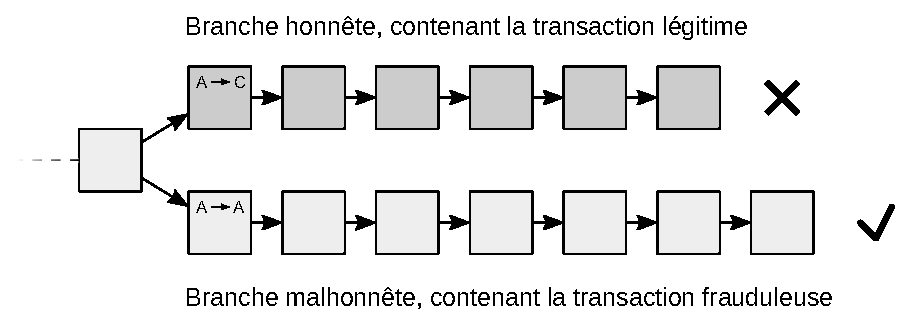
\includegraphics[scale=0.7]{img/mining-attack-doublespending.eps}
  \caption{Attaque de double dépense par recoordination de chaîne.}
  \label{fig:doublespending-attack}
\end{figure}

Il s'agit d'une attaque opportuniste~: elle est motivée par un gain, c'est-à-dire le bien économique obtenu, qui doit être supérieur au coût (matériel, logistique, électrique et logiciel) nécessaire pour y procéder. Sur le réseau Bitcoin principal, ce coût se chiffre aujourd'hui en milliards de dollars\sendnote{Braiins, \eng{How Much Would it Cost to 51\% Attack Bitcoin?}, 11 janvier 2021~: \url{https://braiins.com/blog/how-much-would-it-cost-to-51-attack-bitcoin}.}.

Cette attaque doit être distinguée de la censure, que nous décrirons dans le chapitre~\ref{ch:censure}, et qui consiste à refuser de confirmer des transactions selon un critère arbitraire. Cette dernière repose en effet sur des incitations \emph{extérieures} à l'économie de Bitcoin, le mineur rationnel n'ayant, au sein du système, aucun intérêt économique à ne pas inclure les transactions payant un taux de frais suffisant dans ses blocs.

% --- Incitation ---

Comme souligné par Satoshi, le système est sécurisé tant que la majorité de la puissance de calcul est associée à des nœuds honnêtes, c'est-à-dire des nœuds qui ne cherchent pas à réaliser des doubles dépenses, ni censurer. La sécurité minière repose donc sur une barrière de sécurité, qui représente la charge financière de l'attaquant pour réaliser une double dépense.

% Procédé économique
Cette barrière n'est pas construite de manière bénévole mais repose sur la récompense du protocole, faisant du minage un procédé essentiellement \emph{économique}. En particulier, la résistance à la double dépense -- à savoir la difficulté à effectuer une attaque de double dépense -- dérive directement du revenu minier total, qui incite les nœuds à rester honnêtes. Tel que l'écrivait Satoshi dans le livre blanc~:

\begin{quote}
«~L'incitation peut contribuer à encourager les nœuds à rester honnêtes. Si un attaquant cupide est capable de réunir plus de puissance de calcul que l'ensemble des nœuds honnêtes, il aura à choisir entre l'utiliser pour escroquer des gens en leur récupérant ses paiements, ou l'utiliser pour générer de nouvelles pièces. Il devrait trouver plus rentable de respecter les règles du jeu, celles-ci lui permettant d'obtenir plus de nouvelles pièces que tous les autres réunis, plutôt que de saper le système et la validité de sa propre richesse\sendnote{Satoshi Nakamoto, \eng{Bitcoin: A Peer-to-Peer Electronic Cash System}, 31 octobre 2008.}.~»
\end{quote}

Non seulement la récompense peut être supérieure au gain d'une attaque de double dépense, mais la valeur des bitcoins servant à réaliser la transaction peut aussi être réduite par ladite attaque. En effet, si l'attaque était amenée à être couronnée de succès, on peut imaginer que les différents acteurs diminueraient leur confiance dans le système, arrêteraient de l'utiliser pour le commerce et cèderaient une partie de leur épargne, faisant baisser le revenu de minage et la valeur d'échange du bitcoin. De plus, la spécialisation du matériel de minage (quand elle existe) alourdit le coût de l'attaque, car ce matériel perd dans ce cas en utilité. D'un point de vue purement opportuniste, il est donc la plupart du temps bien plus rentable d'utiliser son capital de manière honnête.

Il est ainsi arrivé que des agrégats de mineurs rassemblent plus de 51~\% de la puissance de calcul, comme la coopérative GHash.io en juillet 2014, sans qu'aucune attaque ne se produise. Et même si une telle attaque avait lieu, celle-ci ne serait pas forcément fatale pour le système à long terme. Comme l'écrivait Satoshi~:

\begin{quote}
«~Même en cas de réussite, cela n'expose pas le système à des modifications arbitraires, comme la création de valeur \emph{ex nihilo} ou l'appropriation d'argent n'ayant jamais appartenu à l'attaquant. Les nœuds ne vont pas accepter une transaction invalide comme paiement, et les nœuds honnêtes n'accepteront jamais un bloc les contenant\sendnote{Satoshi Nakamoto, \eng{Bitcoin: A Peer-to-Peer Electronic Cash System}, 31 octobre 2008.}.~»
\end{quote}

Ainsi de nombreuses attaques de ce type ont déjà eu lieu sur certaines variantes de Bitcoin au fil des années, réduisant leur réputation au passage, mais sans qu'elles ne soient pour autant anéanties. On peut notamment citer Ethereum Classic qui a subi plusieurs recoordinations agressives entre 2019 et 2020\pagenote{«~Ethereum Classic qui a subi plusieurs recoordinations agressives entre 2019 et 2020~»~: Plus précisément~: le 7 janvier 2019, le 31 juillet 2020, le 6 août 2020 et le 29 août 2020.}.

\vspace{-1em}
\section*{L'industrie minière}
\addcontentsline{toc}{section}{L'industrie minière}

Le minage est une activité économique à part entière, la récompense de minage servant à rémunérer le service apporté par le mineur. Cette récompense paie pour le coût de l'électricité, de l'infrastructure matérielle et logistique, et de la maintenance logicielle. Elle compense le risque de production de blocs orphelins. Elle rémunère la confirmation des transactions censurées. Et enfin elle récompense la renonciation temporaire à la liquidité (intérêt originaire du prêteur) et le risque économique général (profit de l'entrepreneur).

Du côté de l'infrastructure matérielle, les mineurs ont besoin de déployer un certain nombre d'éléments~: les machines de hachage (systèmes de refroidissement compris) pour procéder aux calculs liés à la preuve de travail, le processeur pour traiter les blocs et vérifier les signatures, la mémoire pour conserver la chaîne (l'historique), l'ensemble des sorties transactionnelles non dépensées (l'état) et la réserve des transactions en attente, la bande passante pour envoyer et recevoir les transactions et les blocs,~etc. Et force est de constater que tout cela s'est industrialisé au fur et à mesure des années.

% Oublis (logistique) :
% - l'absolue nécessité de pouvoir se relocaliser;
% - la nécessité de disposer d'installation électrique pointue (voire d'en faire construire, via groupes, transformateurs ou centrales électriques);
% - la main d'oeuvre;
% - l'entretien;
% - la réparation;
% - les ingénieurs derrière la pool;
% - les developpeurs et ingénieurs en lien avec les entreprises énergétiques de la grille électrique (Texas), qui développent des logiciels qui viennent à downclock les machines en fonction des besoins.

% --- Industrialisation ---

L'amélioration de la machine pour procéder au hachage illustre bien cette industrialisation. Initialement les mineurs minaient avec le processeur central (CPU) de leur ordinateur. Puis, en 2010, sous l'impulsion de Laszlo Hanyecz puis d'ArtForz, le minage par processeur graphique (GPU) s'est développé. En 2011, est apparu le premier circuit logique programmable FPGA consacré au minage, qui donnait un meilleur rendement que les cartes graphiques\pagenote{«~En 2011, est apparu le premier circuit logique programmable FPGA consacré au minage~»~: fpgaminer, \eng{Official Open Source FPGA Bitcoin Miner (Spartan-6 Now Tops Performance per \$!)}, \wtime{20/05/2011 02:33:56 UTC}~: \url{https://bitcointalk.org/index.php?topic=9047.msg130885\#msg130885}.}. Enfin, en 2013, les premiers circuits intégrés spécialisés (ASIC) ont été mis sur le marché, avec la sortie de l'Avalon ASIC\pagenote{«~la sortie de l'Avalon ASIC~»~: ngzhang, \eng{"Avalon" ASIC, announcement \& pre-order}, \wtime{17/09/2012 07:48:26 UTC}~: \url{https://bitcointalk.org/index.php?topic=110090.msg1197494\#msg1197494}.}. À partir de là, les ASIC sont devenus de plus en plus performants, notamment par le travail de l'entreprise chinoise Bitmain sur ses Antminers.

% L'idée d'utiliser un GPU flottait dans la communauté\sendnote{SmokeTooMuch, \eng{Re: A few suggestions}, \wtime{12/12/2009 13:08:17 UTC}~: \url{https://bitcointalk.org/index.php?topic=12.msg52\#msg52}.}.

Certains acteurs se sont mis à miner de manière industrielle en entassant cette puissance de hachage dans des grands entrepôts spécialisés contenant des centaines de machines, appelés des fermes de minage. Ces fermes ont été installées dans des endroits suivant des facteurs spécifiques dont notamment le coût de l'électricité, la température (coût du refroidissement), la bande passante et l'instabilité politique. Cette émergence de fermes de minage composées d'appareils spécialisés avait été prévue par Satoshi qui écrivait dès novembre 2008~:

\begin{quote}
«~Au début, la plupart des utilisateurs feront fonctionner des nœuds de réseau, mais à mesure que le réseau grandira, au-delà d'un certain point, cette tâche sera de plus en plus déléguée à des spécialistes possédant des fermes de serveurs composées de matériel spécialisé. Une ferme de serveurs n'aura besoin que d'un seul nœud sur le réseau et le reste du réseau local sera connecté à ce nœud\sendnote{Satoshi Nakamoto, \eng{Re: Bitcoin P2P e-cash paper}, \wtime{03/11/2008, 01:37:43 UTC}~: \url{https://www.metzdowd.com/pipermail/cryptography/2008-November/014815.html}.}.~»
\end{quote}

% At first, most users would run network nodes, but as the network grows beyond a certain point, it would be left more and more to specialists with server farms of specialized hardware. A server farm would only need to have one node on the network and the rest of the LAN connects with that one node.

La puissance de calcul du réseau a par conséquent explosé. Le taux de hachage\sendnote{La puissance de hachage apparente $P$ du réseau sur une période donnée peut être retrouvée grâce aux informations de la chaîne que sont la difficulté $d$ et le temps de bloc moyen $\Delta t$. La formule est~: \[
P = \frac{T}{\Delta t} = \frac{1}{\Delta t} \left( \frac{2^{256}}{\frac{C_{\mathrm{max}}}{d} + 1} \right)~.
\] où $T$ est le travail d'un bloc et $C_{\mathrm{max}} = \mathtt{0x00ffff} \times 256^{26}$ est la valeur cible maximale du réseau.}, mesuré en hachages par secondes (H/s), a ainsi connu une spectaculaire croissance au cours des années. En 2009, il oscillait entre 1 et 7 millions de hachage par seconde (1~MH/s). Durant la première partie de 2010, il a progressé pour atteindre les 200~MH/s début juillet. Puis, il a connu deux hausses majeures coïncidant avec les engouements spéculatifs mais aussi avec l'utilisation de méthodes optimisées. La première a été celle de 2010--2011 où le prix est passé de moins d'un centime à 30~\$ et où les premières fermes de cartes graphiques ont été utilisées~: entre juillet 2010 et août 2011, le taux de hachage est passé de 200~MH/s à 15~TH/s (soit une multiplication par 75~000). La seconde a été celle de 2013--2014, période durant laquelle le prix a été quasiment multiplié par 100 et où les premiers ASIC ont été déployés~: le taux de hachage est passé de 25~TH/s en janvier 2013 à 300~PH/s en décembre 2014 (soit une multiplication par 12~000). Le taux de hachage a enfin lentement progressé pour atteindre environ 450~EH/s en novembre 2023 (ce qui correspond à une multiplication par 1~500 depuis décembre 2014).

% --- Délégation de la sélection des transactions (coopératives) ---

Avec cette croissance énorme de la puissance de calcul, la difficulté du minage a suivi. Dès 2010, il devenait difficile d'espérer miner un bloc avec le processeur de son ordinateur. Cela a eu pour effet de désavantager les petits mineurs. L'augmentation de la difficulté a mis en évidence un défaut inhérent du minage~: le défaut de variance. Puisque le minage est soumis aux probabilités, le mineur individuel doté d'un ASIC performant peut ne pas trouver de bloc du tout, tout comme il peut trouver plus de blocs que prévu, faisant reposer son revenu sur le hasard.

C'est pour corriger ce défaut de variance que sont nées les coopératives de minage (appelées \eng{mining pools} en anglais). Ces dernières sont des regroupements de hacheurs qui délèguent leur pouvoir sur la sélection des transactions à un opérateur, afin de participer de manière commune à l'effort de calcul et de lisser leurs revenus. Le fonctionnement par coopératives se base sur la production de preuves de travail partielles (PPoW) mise en place par le protocole Stratum. Il s'agit pour le hacheur de produire une preuve de travail de degré moindre pour un bloc candidat donné, afin de prouver qu'il a dépensé de l'énergie et d'être rémunéré en conséquence par la coopérative. La coopérative reçoit la récompense de minage à chaque fois qu'une preuve de travail partielle produite par le hacheur s'avère être également une preuve de travail complète (FPoW).

% Les coopérative ssont sujettes aux attaques par rétention de bloc (diffusion des PPoW mais pas des FPoW)

La première coopérative de minage a été lancée le 27 novembre 2010 par Marek Palatinus (aussi connu sous le pseudonyme de \eng{slush}). Elle portait initialement le nom de Bitcoin.cz Mining avant d'être plus tard rebaptisée Slush Pool en hommage à son fondateur, puis de devenir Braiins Pool en septembre 2022. Aujourd'hui, les coopératives de minage sont nombreuses et concentrent l'essentiel de la puissance de calcul du réseau. Elles sont généralement basées dans les juridictions où le minage est très présent, comme la Chine (jusqu'en 2021) ou plus récemment les États-Unis.

Les coopératives ont pour habitude de signaler les blocs qu'elles minent dans un souci de transparence. Par exemple, la transaction de récompense du bloc 751~005 contient la chaîne de caractères \longstring{poolin.com}, ce qui indique que ce bloc a très probablement été validé par la coopérative chinoise Poolin. Ce signalement n'est pas obligatoire (le minage est anonyme par essence), mais permet d'avoir une idée de la répartition des différentes coopératives (comme on peut le voir sur la figure~\ref{fig:hashrate-distribution}) et d'estimer par conséquent la centralisation de l'activité minière.

% Foundry USA Pool (USA), Antpool (Chine), F2Pool (Chine), Binance (Chypre ?), ViaBTC (Chine), Slush (République Tchèque), Poolin (Chine), etc.

\begin{figure}[h]
  \centering
  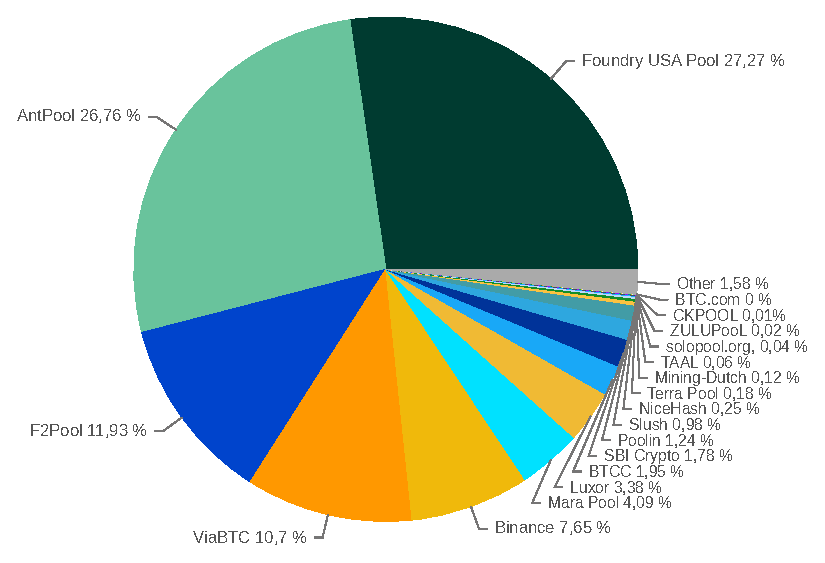
\includegraphics[scale=0.75]{img/hashrate-distribution-coin-dance-week-20231012.eps}
  \caption{Répartition du taux de hachage apparent entre les coopératives de minage de BTC, semaine du 5 au 12 octobre 2023. (source~: coin.dance)}
  \label{fig:hashrate-distribution}
\end{figure}

% --- Délégation de la communication pair à pair (relais) ---

Un autre défaut inhérent du minage est la latence liée à l'annonce des blocs. Comme expliqué dans la section sur la chaîne la plus longue, cette latence produit des blocs orphelins, qui sont valides mais ne sont pas rattachés à la chaîne principale. Cela fait que des mineurs mal connectés ont une puissance de hachage apparente inférieure à leur puissance de hachage réelle.

Pour tenter d'atténuer les effets de ce défaut, les mineurs ont mis en place des relais de communication permettant de s'envoyer des blocs mutuellement de manière plus efficace en supprimant les protections contre le déni de service nécessaires sur le réseau pair à pair ouvert.

Le premier relai a été créé par Matt Corallo sous le nom de \eng{Bitcoin Relay Network}. Il a été lancé en 2013\pagenote{«~Le premier relai [...] a été lancé en 2013~»~: \url{https://lists.linuxfoundation.org/pipermail/bitcoin-dev/2013-November/003596.html}.} et est devenu pleinement fonctionnel en 2015\pagenote{«~[il] est devenu pleinement fonctionnel en 2015~»~: \url{https://web.archive.org/web/20150628233706/https://bitcoinrelaynetwork.org/}.}. Le réseau était composé de plusieurs nœuds spécialisés hébergés sur l'infrastructure Amazon Web Services. Un concurrent était le réseau Falcon, géré par une équipe de l'université Cornell dirigée par Emin Gün Sirer\pagenote{«~Un concurrent était le réseau Falcon~»~: \url{https://web.archive.org/web/20160609081540/https://www.falcon-net.org/}}. Le Bitcoin Relay Network a été remplacé en 2016 par le réseau FIBRE\sendnote{Matt Corallo, \eng{The Future of The Bitcoin Relay Network(s)}, 7 juillet 2016~: \url{https://bluematt.bitcoin.ninja/2016/07/07/relay-networks/}.} (pour \eng{Fast Internet Bitcoin Relay Engine}), un réseau basé sur UDP (protocole alternatif à TCP) qui implémente l'optimisation \texttt{cmpctblock}, toujours géré par Matt Corallo. C'est ce réseau qui est utilisé par la plupart des mineurs aujourd'hui.

% --- Centralisation ---

Cette industrialisation du minage a mené à la centralisation de l'activité minière, à la fois au niveau de la puissance de hachage (fermes de minage) que de la sélection des transactions (coopératives et relais). Si cette agrégation n'est pas fatale (les hacheurs sont libres de quitter leur coopérative pour une autre et les mineurs sont libres de ne pas utiliser le relai), elle n'en diminue pas moins la sécurité minière de la chaîne.

% P2Pool
Certaines améliorations ont été proposées dans le minage pour corriger ce problème. La première est le protocole P2Pool, qui est un protocole de minage coopératif basé sur un réseau pair à pair de mineurs\pagenote{«~P2Pool qui est un protocole de minage coopératif basé sur un réseau pair à pair de mineurs~»~: \url{http://p2pool.in/}.}. Celui-ci met en communication les hacheurs en se basant sur une chaîne latérale -- la «~chaîne de partage~» -- dont la difficulté est plus faible et qui regroupe les différentes contributions des participants. Le développement de P2Pool sur la version principale de Bitcoin semble avoir été mis en suspens en 2017. Toutefois, le procédé est mis en œuvre sur Monero depuis octobre 2021 au moyen d'une coopérative du même nom\pagenote{«~le procédé est mis en œuvre sur Monero~»~: \url{https://p2pool.io/}.}.

% Stratum V2
Le seconde est le protocole Stratum V2\sendnote{Braiins, \eng{Stratum V2 Protocol Overview}~: \url{https://braiins.com/stratum-v2\#job-selection}.}, qui permet (entre autres) aux hacheurs de négocier le contenu des blocs. À défaut de corriger complètement la délégation sur la sélection des transactions, cette nouvelle version de Stratum a le mérite de rendre le processus plus transparent. En novembre 2023, elle n'était déployée qu'au sein de la coopérative Braiins Pool (anciennement Slush Pool), qui est à l'origine de sa conception.

% Limites
Cependant, ces propositions d'amélioration, bien que louables, ne suppriment pas l'avantage économique découlant de la centralisation, qui se retrouve par ailleurs dans toutes les industries (économie d'échelle). La décentralisation a un coût, et celui-ci ne sera justifié que lorsque le bénéfice apporté le surpassera, c'est-à-dire le jour où le réseau sera réellement attaqué.

\section*{Un algorithme de consensus novateur}
\addcontentsline{toc}{section}{Un algorithme de consensus novateur}

Pour fonctionner en tant que système distribué de monnaie numérique, Bitcoin se base sur un mécanisme de consensus novateur. Celui-ci met en jeu une chaîne de blocs construite par les mineurs, qui sont rémunérés pour leur travail. Chaque bloc est un ensemble horodaté de transactions, qui contient une preuve de travail quantifiant l'énergie dépensée. Le consensus est atteint par la sélection de la plus longue chaîne.

Cet algorithme de consensus a un fonctionnement objectif, ouvert et robuste, ce qui explique le succès de Bitcoin par rapport à ses prédécesseurs. Par son aspect essentiellement économique, il donne au système une très grande résistance à la double dépense opportuniste, notamment grâce à la gigantesque industrie minière qui le soutient.

Il existe cependant une menace plus importante, plus insidieuse~: celle de la censure, dont nous parlerons dans le prochain chapitre.
